




\documentclass[10pt, aspectratio=169]{beamer}




\usetheme{default}
\usecolortheme{dove}


\definecolor{azulprimario}{RGB}{37,99,155}
\definecolor{azuloscuro}{RGB}{22,60,100}
\definecolor{azulclaro}{RGB}{220,235,248}
\definecolor{grisoscuro}{RGB}{55,60,67}
\definecolor{grismedio}{RGB}{140,150,160}
\definecolor{grisclaro}{RGB}{243,245,248}


\setbeamerfont{frametitle}{series=\bfseries,size=\Large}
\setbeamerfont{title}{series=\bfseries,size=\LARGE}
\setbeamerfont{block title}{series=\bfseries,size=\normalsize}


\setbeamertemplate{navigation symbols}{}
\setbeamertemplate{blocks}[rounded][shadow=false]
\setbeamertemplate{itemize items}[circle]
\setbeamertemplate{enumerate items}[default]
\setbeamertemplate{section in toc}[sections numbered]
\setbeamertemplate{subsection in toc}[subsections numbered]


\setbeamertemplate{frametitle}{
    \vspace{0.2em}
    \begin{beamercolorbox}[sep=0.2cm,wd=\paperwidth,leftskip=0.3cm]{frametitle}
        \usebeamerfont{frametitle}\insertframetitle
    \end{beamercolorbox}
    \vspace{-0.7em}
    \begin{beamercolorbox}[wd=\paperwidth,ht=0.5pt]{lower separation line head}
    \end{beamercolorbox}
}


\setbeamercolor{structure}{fg=azulprimario}
\setbeamercolor{frametitle}{fg=azuloscuro, bg=white}
\setbeamercolor{lower separation line head}{bg=azulprimario}
\setbeamercolor{title}{fg=azuloscuro, bg=white}
\setbeamercolor{subtitle}{fg=grismedio}
\setbeamercolor{author}{fg=grisoscuro}
\setbeamercolor{date}{fg=grismedio}
\setbeamercolor{institute}{fg=grismedio}


\setbeamercolor{block title}{bg=azulprimario, fg=white}
\setbeamercolor{block body}{bg=azulclaro, fg=grisoscuro}

\setbeamercolor{item}{fg=azulprimario}
\setbeamercolor{footline}{fg=grismedio, bg=white}


\setbeamertemplate{footline}{}


\AtBeginSection[]{
  \begin{frame}[plain]
    \vfill
    \centering
    {\LARGE\bfseries\textcolor{azuloscuro}{\insertsectionhead}}
    \vfill
  \end{frame}
}




\usepackage[spanish]{babel}
\usepackage[utf8]{inputenc}
\usepackage[T1]{fontenc}
\usepackage{lmodern}
\usepackage{amsmath, amssymb}
\usepackage{graphicx}
\usepackage{booktabs}
\usepackage{multirow}
\usepackage{array}
\usepackage{xcolor}
\usepackage{colortbl}
\usepackage{pifont}
\usepackage{makecell}
\usepackage{adjustbox}

\graphicspath{{../codigos_figuras/figures/}}




\title[Parametrización de sinapsis químicas]{Parametrización del modelo de sinapsis química para circuitos neuronales biohíbridos}
\author{Marco Gómez Hernández}
\institute{Escuela Politécnica Superior — Universidad Autónoma de Madrid}
\date{\small Tutor: Pablo Varona Martínez\\ \vspace{0.3em} Departamento: Grupo de Neurocomputación Biológica\\ \vspace{0.3em} \scriptsize mayo 2026}




\begin{document}




\begin{frame}[plain]
    \titlepage
\end{frame}




\begin{frame}{Índice}
    \tableofcontents
\end{frame}


\section{Contexto, motivación y objetivos}



\begin{frame}{Contexto: circuitos neuronales biohíbridos}
    \begin{block}{¿Qué son?}
        \textbf{Neuronas biológicas} y \textbf{modelos neuronales computacionales} interactuando en \textbf{\textit{Hard Real-Time}} (tiempo real estricto).
    \end{block}
    \vspace{0.8em}
    \begin{itemize}
        \item Interacción mediante \textbf{modelos sinápticos computacionales}, cuyos \textbf{parámetros} definen la dinámica del acomplamiento. Modelo estudiado: \textbf{sinapsis química gradual de Golowasch et al.}.
        \item \textbf{\textit{Dynamic Clamp}}: interacción en lazo cerrado.
    \end{itemize}
\end{frame}


\begin{frame}{Problema: parametrización sináptica manual}
    \begin{itemize}
        \item Cada neurona viva es distinta y los \textbf{parámetros no son reutilizables} entre ellas $\to$ \textbf{repetir parametrización} en cada experimento.
        \item \textbf{Muchos parámetros acoplados funcionalemnte} (\textit{parameter sloppiness}) $\to$ parametrización \textbf{lenta} y \textbf{compleja}.
    \end{itemize}
    \vspace{0.8em}
    Cada preparación tiene un \textbf{tiempo de vida limitado} $\to$ \textbf{incompatible}.
    \vspace{0.8em}
    \begin{block}{Necesidad}
        \textbf{Algoritmo} de parametrización \textbf{eficiente} (en número de evaluaciones) y \textbf{adaptado} $\to$ algoritmo de \textbf{optimización de caja negra}.
    \end{block}
\end{frame}




\begin{frame}{Elección del algoritmo de optimización de caja negra}
    \begin{table}
        \centering
        \small
        \begin{tabular}{l >{\centering\arraybackslash}m{3.2cm} c >{\centering\arraybackslash}m{2.0cm}}
            \toprule
            \textbf{Algoritmo}                      & \textbf{Eficiencia en número de evaluaciones} & \textbf{Anti-\textit{parameter sloppiness}}    & \textbf{Convergencia global}                   \\
            \midrule
            Nelder-Mead                             & Media                                         & \textcolor{red!70!black}{\ding{55}}            & \textcolor{red!70!black}{\ding{55}}            \\
            Algoritmos genéticos                    & \textcolor{red!70!black}{Baja}                & \textcolor{red!70!black}{\ding{55}}            & \textcolor{green!50!black}{\ding{51}}          \\
            PSO                                     & \textcolor{red!70!black}{Baja}                & \textcolor{red!70!black}{\ding{55}}            & \textcolor{green!50!black}{\ding{51}}          \\
            CMA-ES                                  & \textcolor{red!70!black}{Baja}                & \textcolor{green!50!black}{\ding{51}}          & \textcolor{green!50!black}{\ding{51}}          \\
            \textbf{\textit{Bayesian Optimization}} & \textcolor{green!50!black}{\textbf{Alta}}     & \textcolor{green!50!black}{\textbf{\ding{51}}} & \textcolor{green!50!black}{\textbf{\ding{51}}} \\
            \bottomrule
        \end{tabular}
    \end{table}
\end{frame}


\begin{frame}{Objetivos}
    \begin{enumerate}
        \item Diseñar una \textbf{función de evaluación} para unos parámetros (morfología + rango de corriente).
        \item Adaptar la \textbf{\textit{Bayesian Optimization}} al modelo sináptico, incluyendo mecanismos anti-\textit{parameter sloppiness}.
        \item Implementación \textbf{\textit{offline}}: parametrización rápida sobre señales pregrabadas en interacción unidireccional.
        \item Implementación \textbf{\textit{online}}: módulo RTXI que parametrice en tiempo real, permitiendo interacción bidireccional.
        \item \textbf{Validar} ambas versiones: corrientes realistas, tiempos viables y corrección del proceso de optimización.
    \end{enumerate}
\end{frame}


\section{Diseño y desarrollo}



\begin{frame}{Modelo neuronal utilizado: Hindmarsh-Rose modificado}
    \begin{equation*}
        \boxed{
            \begin{aligned}
                \frac{d\boldsymbol{x(t)}}{dt} & = y(t) + b x^2(t) - a x^3(t) - z(t) + e - \boldsymbol{I_{\mathrm{syn}}(t)} \\[3pt]
                \frac{dy(t)}{dt}              & = c - d x^2(t) - y(t)                                                      \\[3pt]
                \frac{1}{\mu}\frac{dz(t)}{dt} & = -v_h \cdot z(t) + S(x(t) - x_r)
            \end{aligned}
        }
    \end{equation*}
    \begin{itemize}
        \item Modelo fenomenológico: reproduce \textbf{\textit{bursting}}.
        \item \textbf{Simplificado}, pero \textbf{suficiente} para el trabajo.
        \item Voltaje \textbf{adimensional}
        \item Valores iniciales y parámetros con sus \textbf{valores comunes}, salvo las modificaciones del GNB de $\boldsymbol{v_h}$ ($1{,}0 \to 0{,}1$) y $\boldsymbol{S}$ ($4{,}0 \to 1{,}0$) $\to$ \textbf{hiperpolarización flexible} y \textbf{ráfagas estables}.
    \end{itemize}
\end{frame}


\begin{frame}
    \vfill
    \centering
    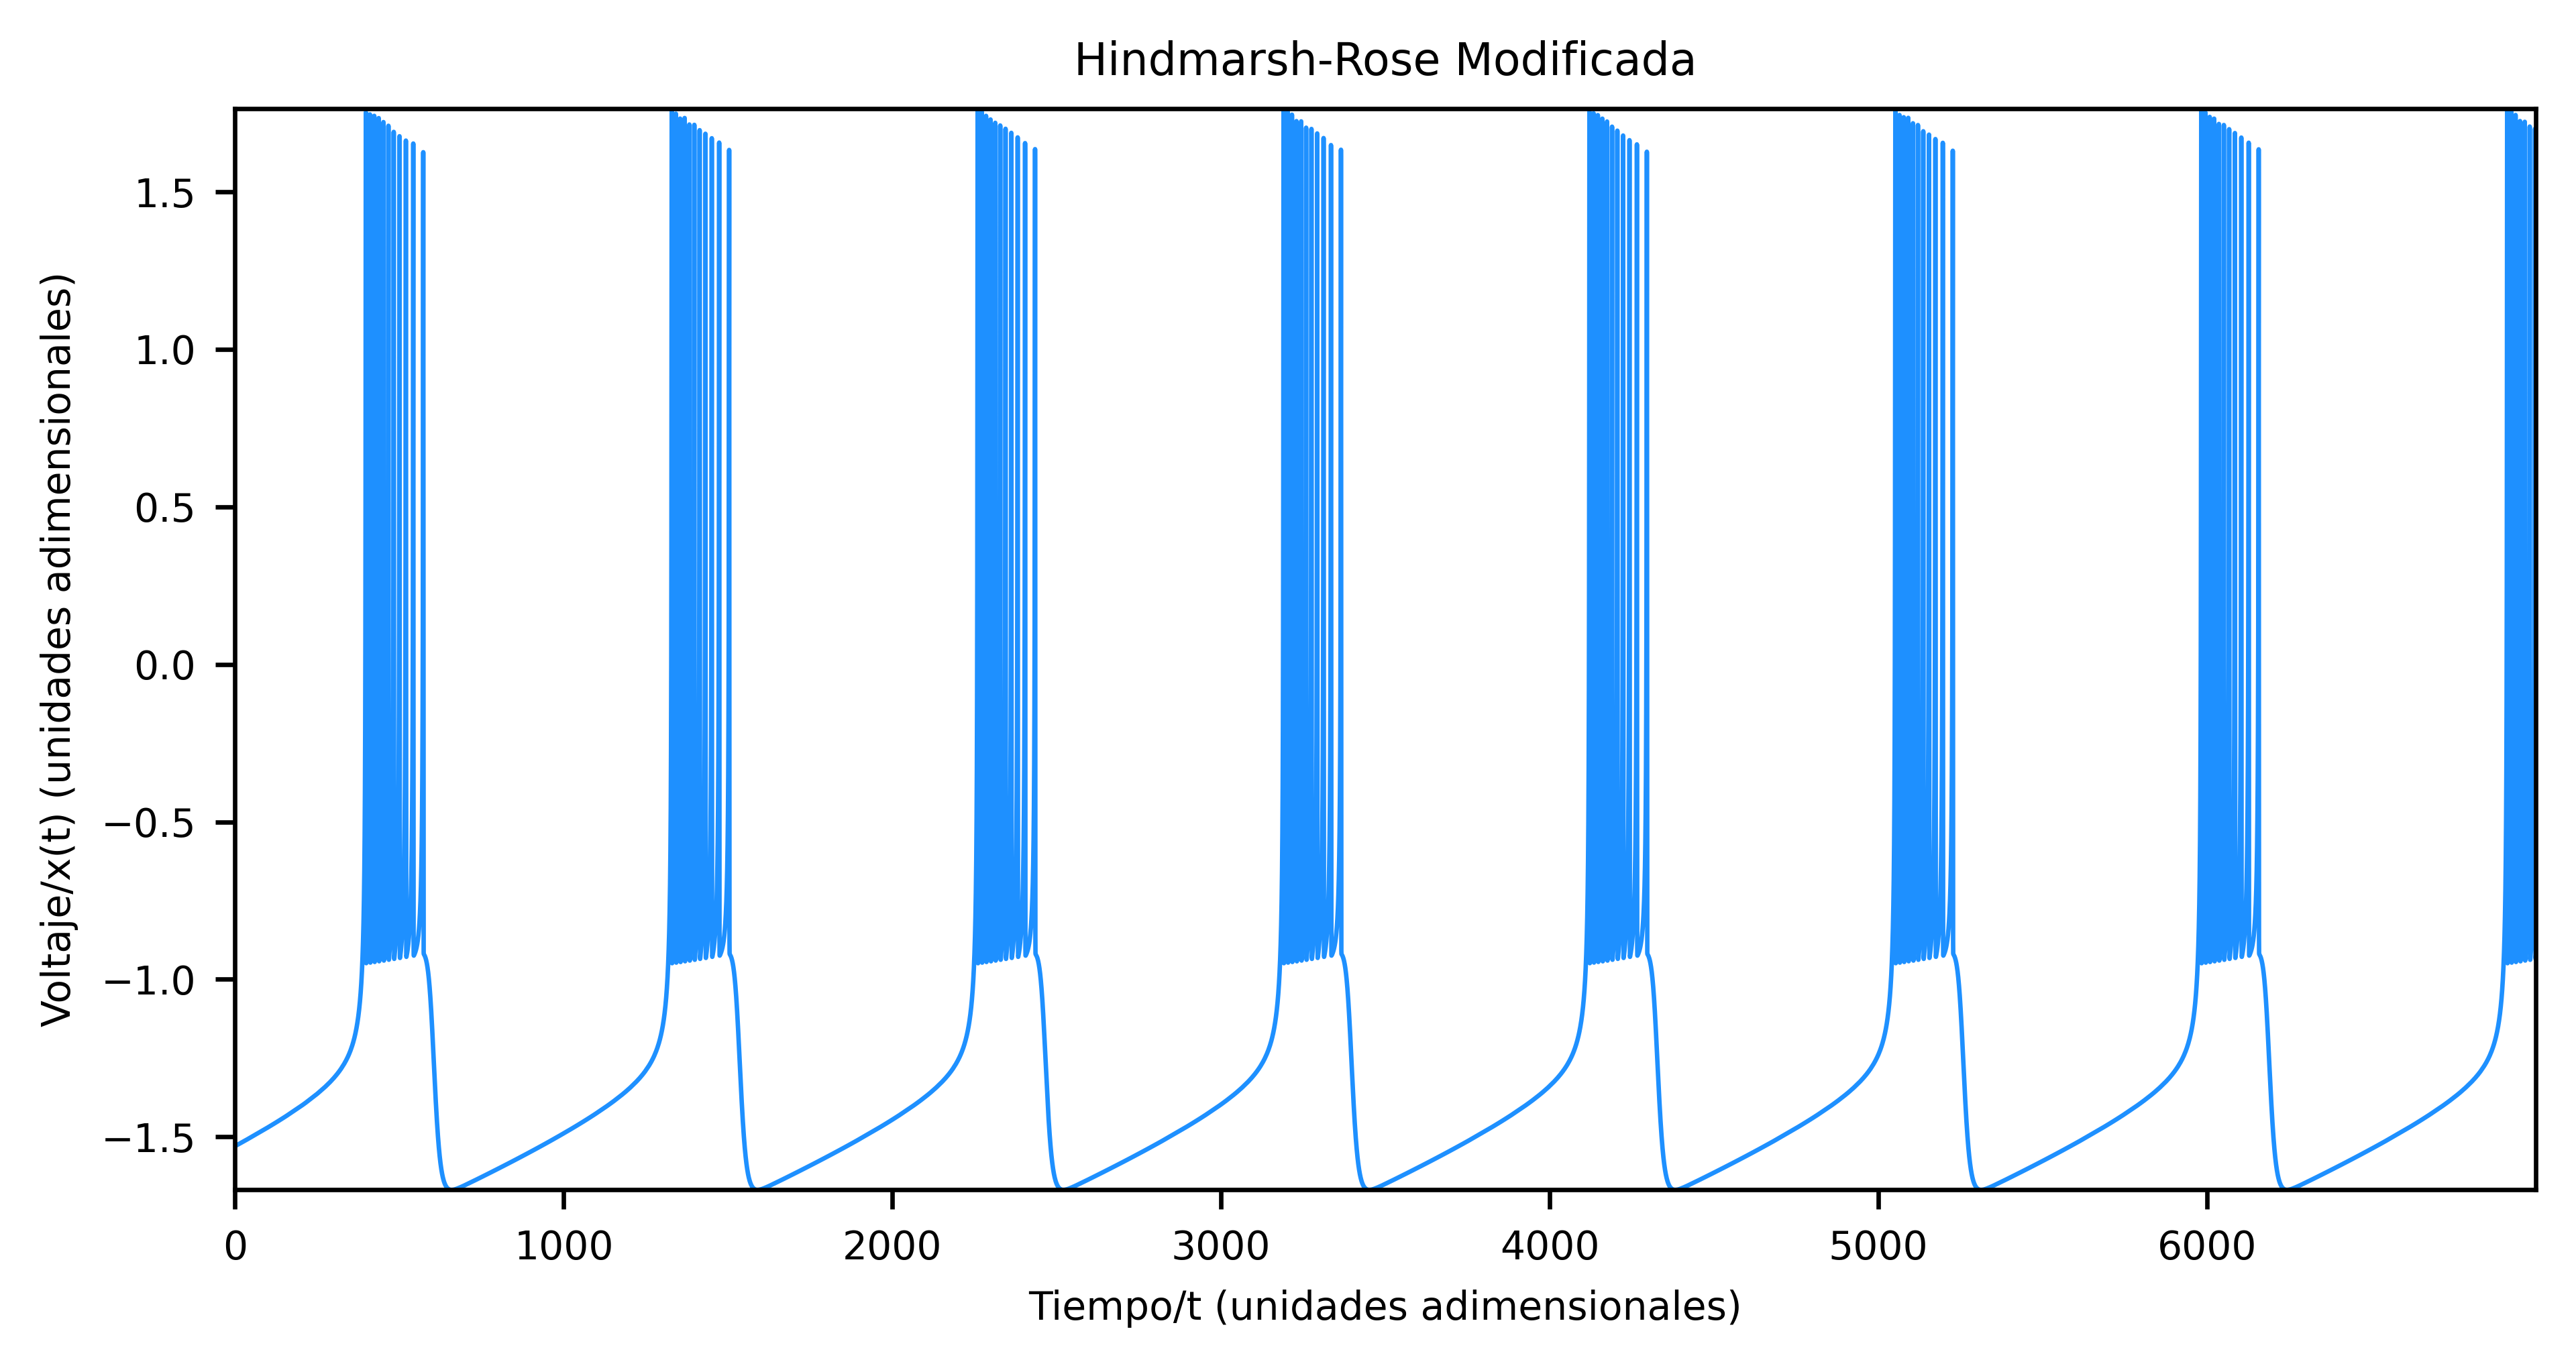
\includegraphics[width=\textwidth, height=\textheight, keepaspectratio]{hindmarsh-rose_modified}
    \vfill
\end{frame}


\begin{frame}{Modelo de sinapsis química gradual de Golowasch et al.}
    \centering
    \scriptsize
    \begin{tabular}{@{} >{\centering\arraybackslash}p{0.45\linewidth} @{\hspace{0pt}} >{\centering\arraybackslash}p{0.45\linewidth} @{}}
        \textbf{Componente rápida} (altas frecuencias/\textit{spikes} de $V_{\mathrm{pre}}$; aunque podría capturar ambas componentes a la vez)                                                                                           &
        \textbf{Componente lenta} (bajas frecuencias de $V_{\mathrm{pre}}$)                                                                                                                                                                 \\[0.8em]
        \adjustbox{valign=T}{$\boxed{\begin{aligned}[t] I_{\mathrm{fast}} = g_{\mathrm{fast}} \cdot \frac{V_{\mathrm{post}} - E_{\mathrm{syn}}}{1 + \exp[ s_{\mathrm{fast}} \cdot (V_{\mathrm{fast}} - V_{\mathrm{pre}}) ]} \end{aligned}}$} &
        \adjustbox{valign=T}{$\boxed{\begin{aligned}[t]
                                                     I_{\mathrm{slow}}              & = g_{\mathrm{slow}} \cdot m_{\mathrm{slow}} \cdot (V_{\mathrm{post}} - E_{\mathrm{syn}})                                                             \\[-2pt]
                                                     \frac{d m_{\mathrm{slow}}}{dt} & = \frac{k_1 \cdot (1 - m_{\mathrm{slow}})}{1 + \exp[ s_{\mathrm{slow}} \cdot (V_{\mathrm{slow}} - V_{\mathrm{pre}}) ]} - k_2 \cdot m_{\mathrm{slow}}
                                                 \end{aligned}}$}
    \end{tabular}

    \vspace{0.8em}
    \fcolorbox{azulprimario}{azulclaro}{\;$\boldsymbol{I_{\mathrm{syn}} = I_{\mathrm{fast}} + I_{\mathrm{slow}}}$\;}

    \vspace{0.8em}
    \setlength{\tabcolsep}{2pt}
    \begin{tabular}{|l|>{\raggedright\arraybackslash}m{3.8cm}|>{\raggedright\arraybackslash}m{2.6cm}|l|l|}
        \hline
        \textbf{Parámetro}       & \textbf{Descripción}                                                                                                                 & \textbf{Escala con}                                                  & \textbf{Unidad}           & \textbf{Valores interesantes}                                         \\
        \hline
        \rowcolor{azulclaro}
        $g_{\mathrm{fast/slow}}$ & Conductancias, controlan amplitud de $I_{\mathrm{fast/slow}}$                                                                        & Rango de $V_{\mathrm{post}}$ inv., $I_{\mathrm{fast/slow}}$ objetivo & $\mathrm{\mu S}$          &                                                                       \\
        \hline
        $E_{\mathrm{syn}}$       & Potencial de reversión, controla si se causa excitación/fase o inhibición/antifase al controlar el signo de $I_{\mathrm{fast/slow}}$ & Rango de $V_{\mathrm{post}}$                                         & mV                        & \makecell[l]{Alejado del rango de $V_{\mathrm{post}}$                 \\\\$>$ rango de $V_{\mathrm{post}}$: excitación/fase\\$<$ rango de $V_{\mathrm{post}}$: inhibición/antifase}                                                             \\
        \hline
        \rowcolor{azulclaro}
        $s_{\mathrm{fast/slow}}$ & Pendientes sigmoides                                                                                                                 & Rango de $V_{\mathrm{pre}}$ inv.                                     & $\mathrm{mV}^{-1}$        & $s_{\mathrm{fast}} > s_{\mathrm{slow}}$                               \\
        \hline
        $V_{\mathrm{fast/slow}}$ & Umbrales sigmoides                                                                                                                   & Rango de $V_{\mathrm{pre}}$                                          & mV                        & \makecell[l]{$V_{\mathrm{fast}}$: valores altos de $V_{\mathrm{pre}}$ \\$V_{\mathrm{slow}}$: valores bajos de $V_{\mathrm{pre}}$} \\
        \hline
        \rowcolor{azulclaro}
        $k_1$                    & Tasa de apertura de $m_{\mathrm{slow}}$                                                                                              & Frecuencia de corte                                                  & $\mathrm{\text{ms}}^{-1}$ &                                                                       \\
        \hline
        $k_2$                    & Tasa de cierre de $m_{\mathrm{slow}}$                                                                                                & Frecuencia de corte                                                  & $\mathrm{\text{ms}}^{-1}$ &                                                                       \\
        \hline
    \end{tabular}
\end{frame}


\begin{frame}{Modelo de sinapsis química gradual de Golowasch et al.}
    \begin{itemize}
        \item Presencia de \textbf{\textit{parameter sloppiness}}: a la \textbf{amplitud} de $I_{\mathrm{fast/slow}}$ le afectan \textbf{todos} los parámetros de cada fórmula.
              \vspace{1.5em}
        \item $I_{\mathrm{syn}}$ se inyecta en la neurona \textbf{postsináptica} $\to$ una sinapsis \textbf{distinta} por dirección.
    \end{itemize}
\end{frame}






\begin{frame}{Función de evaluación de los parámetros}
    \small
    Uso de las altas y bajas \textbf{frecuencias de} $\boldsymbol{V_{\mathrm{pre}}}$ (en un intervalo de evaluación) como \textbf{referencia de las corrientes generadas con unos parámetros} (en el mismo intervalo) $\to$ \textbf{filtro paso bajo sobre} $\boldsymbol{V_{\mathrm{pre}}}$ con la librería KFR:
    \begin{itemize}
        \item Butterworth de 4.º orden.
        \item Fase cero.
        \item Función de transferencia en SOS.
    \end{itemize}
    Requiere \textit{padding}.
\end{frame}


\begin{frame}{Función de evaluación de los parámetros}
    \centering
    \begin{columns}[t]
        \begin{column}{0.48\textwidth}
            \begin{block}{Puntuación de forma}
                \small
                \textbf{Coeficiente de correlación de Pearson} normalizado en $[0, 1]$:
                \begin{itemize}
                    \item \textbf{Antifase} $\to$ \textbf{correlación}.
                    \item \textbf{Fase} $\to$ \textbf{correlación negativa}.
                \end{itemize}
            \end{block}
        \end{column}
        \begin{column}{0.48\textwidth}
            \begin{block}{Puntuación de rango}
                \scriptsize
                \begin{equation*}
                    \mathrm{score}_{\mathrm{rango}} = 1 - \frac{\frac{1}{2}(|\Delta I_{\min}| + |\Delta I_{\max}|)}{d_{\max}}
                \end{equation*}
                \begin{itemize}
                    \item Resultado en $\boldsymbol{[-\infty, 1]}$, normalmente $\ge 0$.
                    \item \textbf{Extremos objetivo}:
                          \begin{itemize}
                              \scriptsize
                              \item Si se usa \textbf{una componente de la corriente}: los introducidos por el usuario.
                              \item Si se usan \textbf{ambas}: escalado de los introducidos por el usuario con los de la referencia (componente rápida hereda amplitud, lenta amplitud y offset).
                          \end{itemize}
                \end{itemize}
            \end{block}
        \end{column}
    \end{columns}
    \vspace{0.8em}
    \fcolorbox{azulprimario}{azulclaro}{\small Puntuación final = media}\par
\end{frame}


\begin{frame}{\textit{Bayesian Optimization}}
    Construye un \textbf{modelo subrogado} del objetivo, un \textbf{GP}. Librería \textbf{Limbo}:
    \begin{columns}[t]
        \begin{column}{0.48\textwidth}
            \begin{itemize}
                \item \textbf{\textit{Kernel} SE-ARD} $\to$ anti-\textit{parameter sloppiness}.
                \item \textbf{Hiperparámetros reoptimizados con Rprop}.
                \item \textbf{Adquisición \textit{EI} con maximización mediante Subplex} (librería NLOpt) $\to$ equilibro exploración-explotación (controlado por \textit{jitter}).
                \item \textbf{Muestras Iniciales LHS} $\to$ cobertura uniforme.
            \end{itemize}
        \end{column}
        \begin{column}{0.48\textwidth}
            \scriptsize
            \begin{block}{Configuraciones del usuario}
                \begin{itemize}
                    \item \textbf{Muestras LHS}.
                    \item \textbf{Iteraciones}.
                    \item \textbf{Componente(s) de la corriente} cuyos parámetros se optimizan (dimensionalidad del problema).
                \end{itemize}
            \end{block}
            \begin{block}{Configuraciones dinámicas automáticas}
                \begin{itemize}
                    \item \textbf{Iteraciones de Rprop}: escala con dimensionalidad.
                    \item \textbf{Re-optimización del GP}: escala con las iteraciones totales.
                    \item \textbf{Iteraciones de Subplex}: escala cuadráticamente con dimensionalidad.
                \end{itemize}
            \end{block}
        \end{column}
    \end{columns}
\end{frame}


\begin{frame}{Estrategias de configuración del espacio de búsqueda}
    \small
    \begin{columns}[t]
        \begin{column}{0.48\textwidth}
            \textbf{Rangos dinámicos adaptados:}
            \begin{itemize}
                \item[] BO opera con los parámetros en $\boldsymbol{[0, 1]}$ $\to$ \textbf{desnormalización} antes de usarlos en el modelo.
                \item[] \textbf{Rangos de desnormalización}: calculados según lo visto, pero $g_{\mathrm{fast/slow}}$ con los extremos de los otros rangos y los de $I_{\mathrm{fast/slow}}$ objetivo (con márgen).
            \end{itemize}
        \end{column}
        \begin{column}{0.48\textwidth}
            \textbf{Medidas anti-\textit{parameter sloppiness}:}
            \begin{itemize}
                \item \textit{Kernel} \textbf{SE-ARD} $\to$ escala de longitud por parámetro.
                \item \textbf{Reparametrización} $\boldsymbol{R = k_2/k_1}$ $\to$ desacoplamiento de la cinética del equilibrio apertura-cierre.
                      \begin{equation*}
                          m_{\mathrm{slow}}^{\infty} = \frac{\sigma_{\mathrm{slow}}(V_{\mathrm{pre}})}{\sigma_{\mathrm{slow}}(V_{\mathrm{pre}}) + R}
                      \end{equation*}
                      \vspace{-0.5em}
                \item \textbf{Escala logarítmica} para $\boldsymbol{g}$, $\boldsymbol{k_1}$, $\boldsymbol{R}$ ($k_2$ la tendría) $\to$ reducción de la anisotropía del espacio (además abarcan varios órdenes de magnitud).
            \end{itemize}
        \end{column}
    \end{columns}
\end{frame}


\begin{frame}{Escalado de la señal presináptica de Reyes-Sanchez et al.}
    \small
    La neurona \textbf{Hindmarsh-Rose} opera en \textbf{unidades adimensionales} de amplitud y tiempo; la \textbf{viva}, en \textbf{reales}.
    \vspace{-1em}
    \begin{columns}[t]
        \begin{column}{0.48\textwidth}
            \begin{block}{Escalado de amplitud}
                \vspace{-1em}
                \begin{equation*}
                    \begin{aligned}
                        \mathrm{factor}       & = \frac{\Delta V_{\mathrm{model}}}{\Delta V_{\mathrm{real}}}               \\
                        \mathrm{offset}       & = V_{\mathrm{model,}\min} - (V_{\mathrm{real,}\min} \cdot \mathrm{factor}) \\
                        V_{\mathrm{escalado}} & = V_{\mathrm{real}} \cdot \mathrm{factor} + \mathrm{offset}
                    \end{aligned}
                \end{equation*}
                \begin{itemize}
                    \item \textbf{Innecesario} si cada parámetro estuviese en la escala de su dependencia (sigmoide y $m_{\mathrm{slow}}$ adimensionales).
                    \item Posible \textbf{\textit{check drift}} $\to$ adaptabilidad a cambios.
                \end{itemize}
            \end{block}
        \end{column}
        \begin{column}{0.48\textwidth}
            \begin{block}{Escalado temporal}
                \begin{enumerate}
                    \item Cálculo de \textbf{datos temporales del \textit{burst}} (histéresis 10\,\% y 90\,\%).
                    \item Evaluación de \textbf{múltiplos crecientes del periodo de \textit{burst} presináptico}
                    \item Búsqueda \textbf{descendente} de $\boldsymbol{dt}$ (mayor eficiencia) hasta que cumpla el \textbf{umbral} del múltiplo y \textbf{divisibilidad}.
                    \item El múltiplo define el \textbf{factor de submuestreo} $\to$ estabilidad Hindmarsh-Rose.
                \end{enumerate}
            \end{block}
        \end{column}
    \end{columns}
    \vspace{1em}
    \textbf{Precálculo} de los datos de la Hindmarsh-Rose para el escalado $\to$ no se repite.
\end{frame}


\begin{frame}{Implementación \textit{offline}}
    \vfill
    \centering
    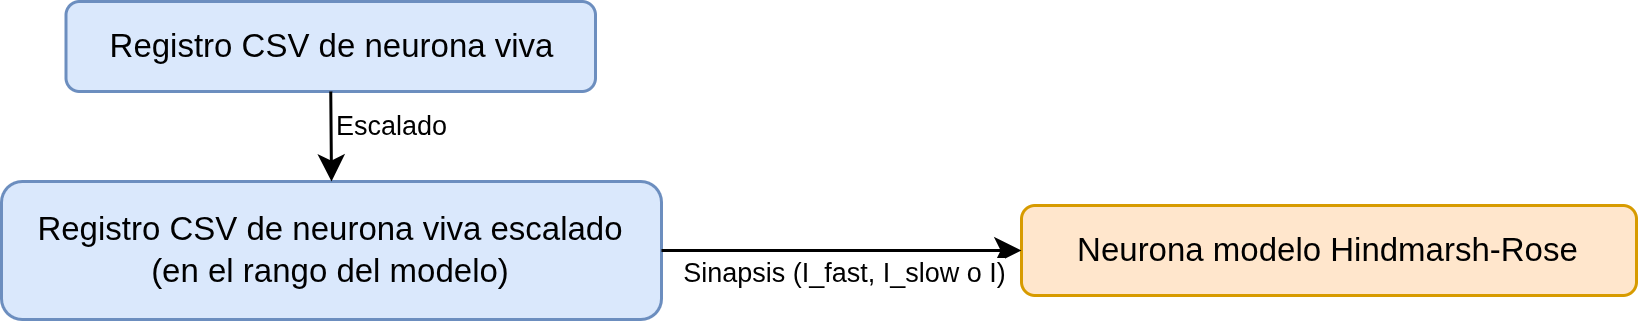
\includegraphics[width=\textwidth, height=\textheight, keepaspectratio]{esquema_neuronas_offline}
    \vfill
\end{frame}


\begin{frame}{Implementación \textit{offline}}
    \scriptsize
    \begin{itemize}
        \item Sin esperas de tiempo real $\to$ \textbf{gran velocidad}.
        \item Registro de una \textbf{neurona PD del ganglio estomatogástrico de un crustáceo} porque presenta el \textit{bursting} típico del \textbf{CPG}.
        \item Integrador \textbf{Runge-Kutta de 4.º orden} $\to$ equilibrio eficiencia-coste.
        \item Mismo fragmento del registro + reinicio de variables de los modelos entre evaluaciones $\to$ \textbf{evaluaciones deterministas} $\to$ \textbf{ruido fijo y reducido} en la BO.
        \item \textbf{Escalado no causal} (señal estática) $\to$ evita sesgos.
        \item \textbf{Interpolación lineal de} $\boldsymbol{V_{\mathrm{pre}}}$ $\to$ suavidad y estabilidad de los modelos.
        \item \textbf{Pasos de estabilización} en los modelos.
        \item {\textbf{Reservas de memoria y cálculos}} que se repetirían se hacen \textbf{una sola vez} $\to$ eficiencia.
        \item Librería de modelos: \textbf{Neun} $\to$ fácil cambio de modelos.
        \item Usuario configura:
              \begin{itemize}
                  \scriptsize
                  \item Muestras iniciales e iteraciones.
                  \item \textbf{Frecuencia de corte}.
                  \item Componentes de la corriente a optimizar y sus extremos objetivo y \textbf{permitidos} (\textit{clamp} para no desestablizar modelos y seguir evaluando).
                  \item Búsqueda de \textbf{fase o antifase}.
                  \item \textbf{Tiempos de estabilización, observación y evaluación}.
              \end{itemize}
    \end{itemize}
\end{frame}


\begin{frame}{Implementación \textit{online}}
    \vfill
    \centering
    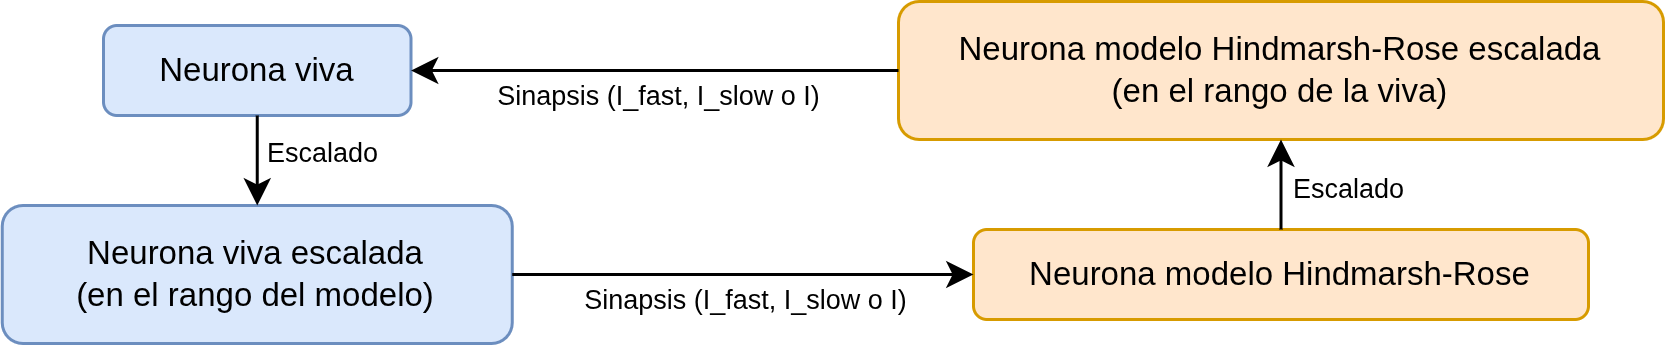
\includegraphics[width=\textwidth, height=\textheight, keepaspectratio]{esquema_neuronas_online}
    \vfill
\end{frame}


\begin{frame}{Implementación \textit{online}}
    \scriptsize
    \begin{itemize}
        \item Módulo para \textbf{RTXI 2.3} (versión del laboratorio).
        \item El módulo agrupa las sinapsis en \textbf{ambas} direcciones (puntuación es la \textbf{media}) $\to$ captura la dinámica completa.
        \item \textbf{Módulo sináptico}, no solo parametriza.
        \item \textbf{Implementación propia del modelo} para calcular solo las corrientes \textbf{seleccionadas} $\to$ \textbf{eficiencia}, crítica en \textbf{tiempo real}.
        \item Integrador \textbf{Runge-Kutta de 5.º orden y 6 etapas} $\to$ equilibrio eficiencia-coste.
        \item $\boldsymbol{dt}$ \textbf{pequeño y propio} (usuario), \textbf{sin submuestreo} (sinapsis no ve el de la neurona). Estable porque $m_{\mathrm{slow}}$ es lineal en su EDO $\to$ estabilidad, aunque aun así se \textit{clampea} $m_{\mathrm{slow}}$ si se sale mucho de rango.
        \item Intervalos distintos por evaluación $\to$ \textbf{evaluaciones no deterministas} $\to$ \textbf{ruido moderado y optimizable} y \textbf{\textit{jitter} bajo} (para no explotar ruido) en la BO.
        \item \textbf{Margen en el rango de} $\boldsymbol{V_\mathrm{pre}}$ usado para calcular los rangos de los parámetros (por si cambia).
        \item Uso de los módulos de \textbf{RTHybrid} para \textbf{RTXI}.
    \end{itemize}
\end{frame}

\begin{frame}{Implementación \textit{online}: hilos}
    \textbf{Tres hilos}:
    \begin{itemize}
        \item \textbf{RT (operaciones ligeras)}: calcula corrientes y recolecta señales para el NRT. Se coordina con el NRT \textbf{sin bloqueos}.
        \item \textbf{NRT (operaciones pesadas)}: hace la optimización, reservas de memoria, actualiza la GUI...  Lanzado con un botón. Se coordina con el RT \textbf{con o sin esperas} y envía eventos \textbf{asíncronos} a la GUI.
        \item \textit{GUI}: recibe eventos asíncronos del NRT y del usuario.
    \end{itemize}
    \vspace{1em}
    Coordinación entre hilos RT y NRT: \textbf{variables atómicas} y \textbf{\textit{double buffering}}. Entre el RT y la GUI, RTXI se encarga.\\[0.5em]
    BO puede \textbf{interrumpirse}, dejando el candidato actual.
\end{frame}


\begin{frame}{Esquema de módulos: dos neuronas modelo}
    \vfill
    \centering
    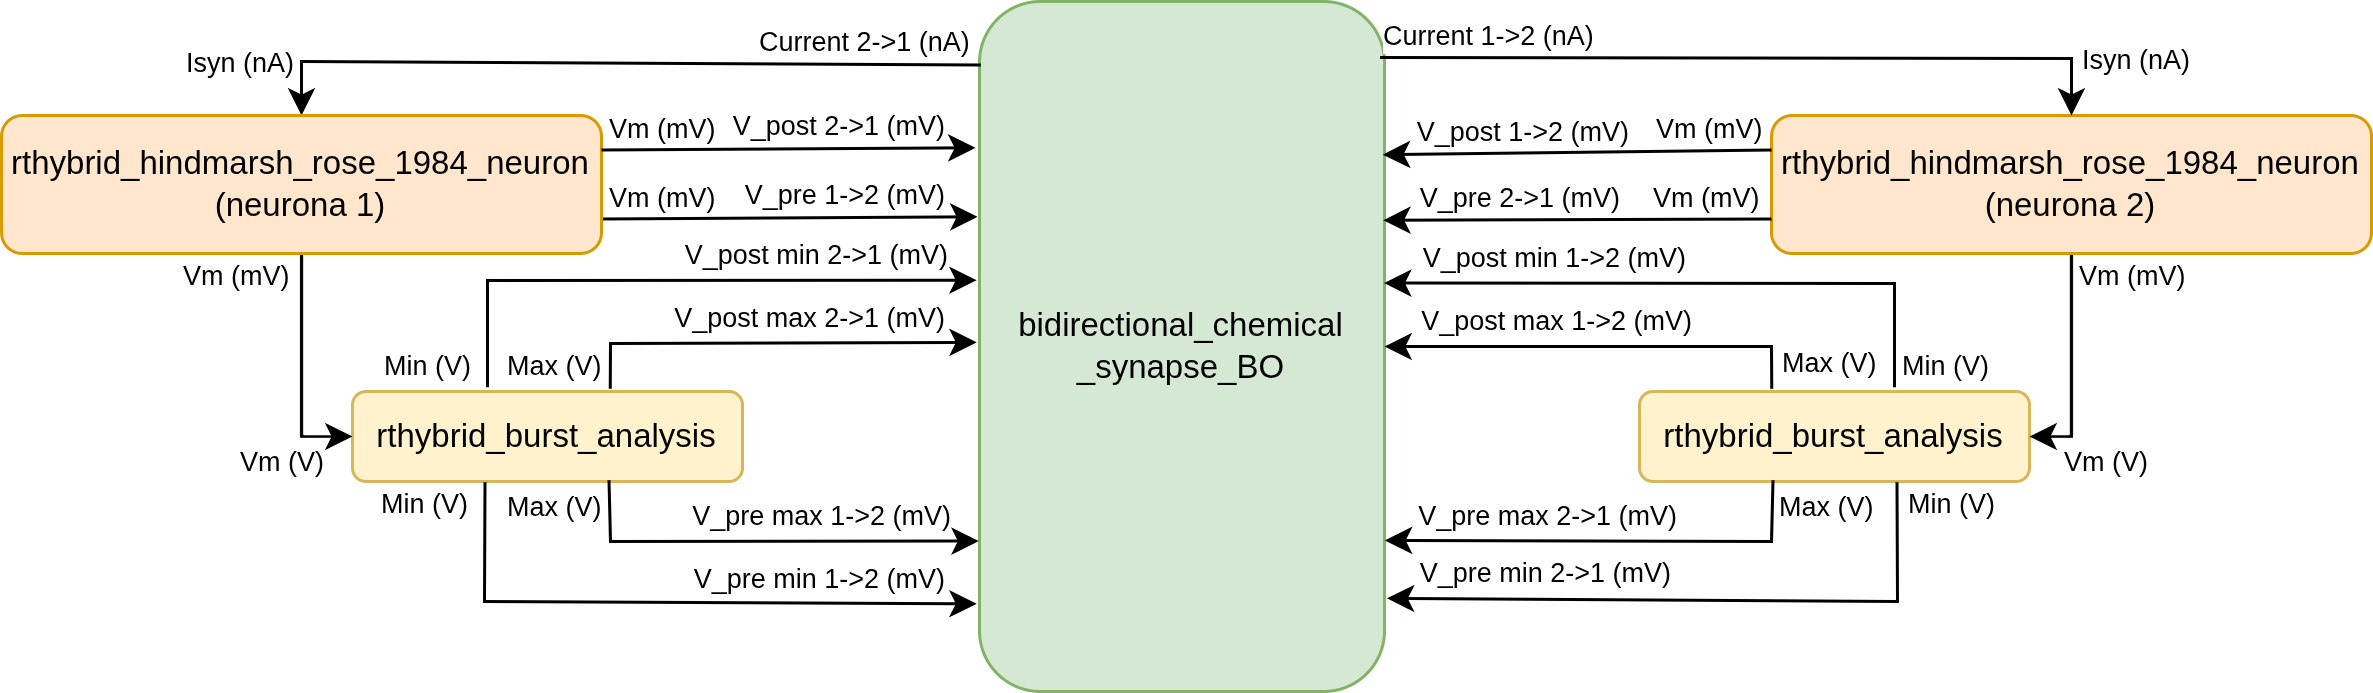
\includegraphics[width=\textwidth, height=\textheight, keepaspectratio]{esquema_modulos_online_modelo}
    \vfill
\end{frame}


\begin{frame}{Esquema de módulos: neurona modelo + viva}
    \vfill
    \centering
    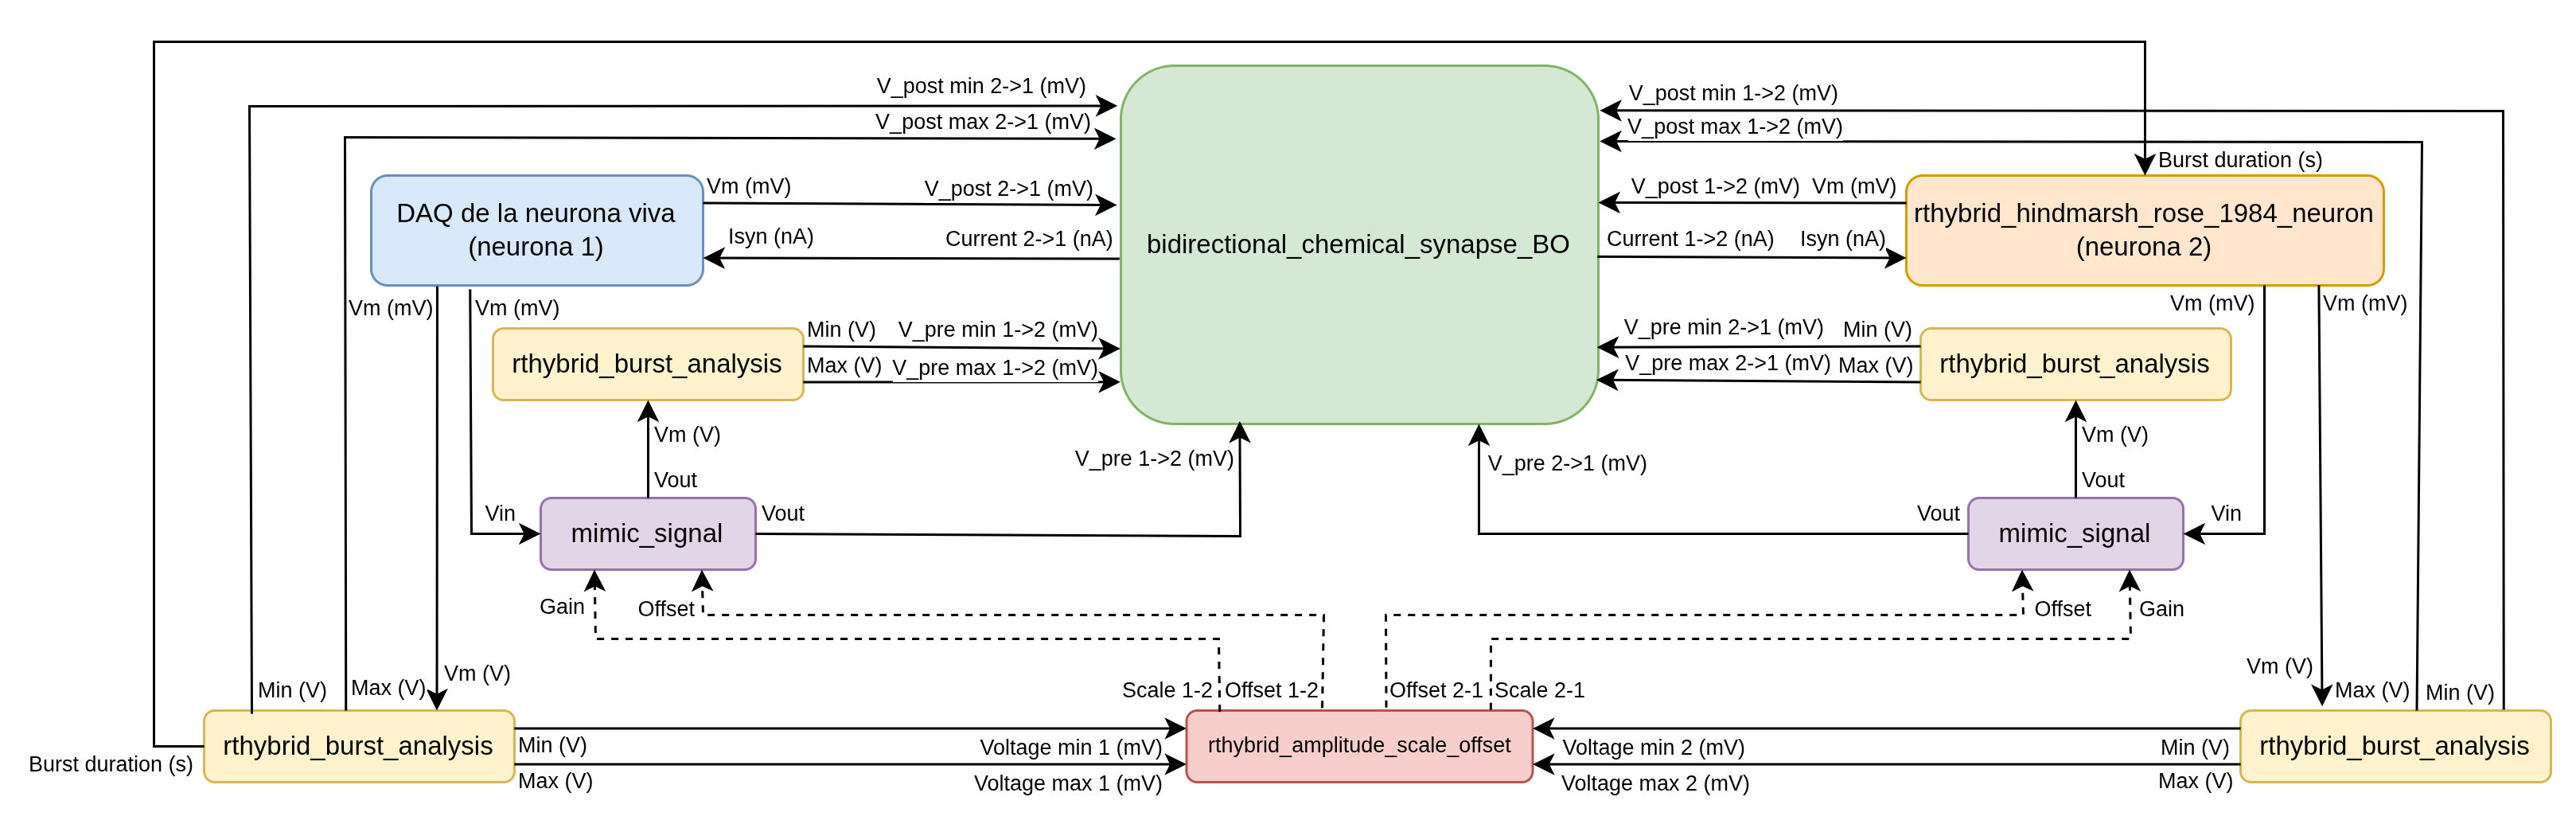
\includegraphics[width=\textwidth, height=\textheight, keepaspectratio]{esquema_modulos_online_viva}
    \vfill
\end{frame}


\section{Resultados}



\begin{frame}{Resultados de la implementación \textit{offline}}
    \scriptsize
    \begin{columns}[t]
        \begin{column}{0.48\textwidth}
            Configuraciones:
            \begin{itemize}
                \item $\boldsymbol{I_{\mathrm{fast}}}$ e $\boldsymbol{I_{\mathrm{slow}}}$ a la vez.
                \item \textbf{50 muestras iniciales + 350 iteraciones = 400 evaluaciones} $\to$ \textbf{suficiente} dada la dimensionalidad (9) y \textbf{no excesivo}.
                \item Estabilización de $4000$\,ms y \textbf{evaluación} y observación de $7000$\,ms ($\boldsymbol{\sim 5}$ \textbf{\textit{bursts}}). Mucho, pero no hay que esperar eso realmente.
                \item Frecuencia de corte de $0{,}024$\,kHz.
                \item Promedio de \textbf{20 ejecuciones} $\to$ \textbf{rigurosidad estadística}.
                \item \textbf{Rangos de corriente objetivo}:
                      \begin{itemize}
                          \scriptsize
                          \item \textbf{Antifase}: $\boldsymbol{[-1{,}4; -0{,}4]}$ u. a..
                          \item \textbf{Fase}: $\boldsymbol{[0{,}2; 0{,}8]}$ u. a..
                      \end{itemize}
            \end{itemize}
        \end{column}
        \begin{column}{0.48\textwidth}
            Resultados:
            \begin{itemize}
                \item Tiempos:
                      \begin{itemize}
                          \scriptsize
                          \item \textbf{Antifase}: $\boldsymbol{29{,}57 \pm 9{,}27}$\,\textbf{s}.
                          \item \textbf{Fase}: $\boldsymbol{32{,}2 \pm 6{,}77}$\,\textbf{s}.
                      \end{itemize}
                \item Parámetros:
                      \begin{itemize}
                          \scriptsize
                          \item $\boldsymbol{g_{\mathrm{fast}} < g_{\mathrm{fast}}}$ porque la \textbf{amplitud de los \textit{spikes} $<$ la de la onda lenta}.
                          \item $\boldsymbol{k_1 < k_2}$, aunque ambas con \textbf{alta variabilidad} $\to$ \textbf{\textit{parameter sloppiness}}.
                          \item $V_{\mathrm{slow}}$ con \textbf{media inesperada y alta variabilidad} $\to$ \textbf{\textit{parameter sloppiness}} (por el pequeño rango de $s_{\mathrm{slow}}$).
                          \item El resto, según lo esperado de forma estable.
                      \end{itemize}
            \end{itemize}
        \end{column}
    \end{columns}
\end{frame}


\begin{frame}{Convergencia de la implementación \textit{offline}: antifase}
    \vfill
    \centering
    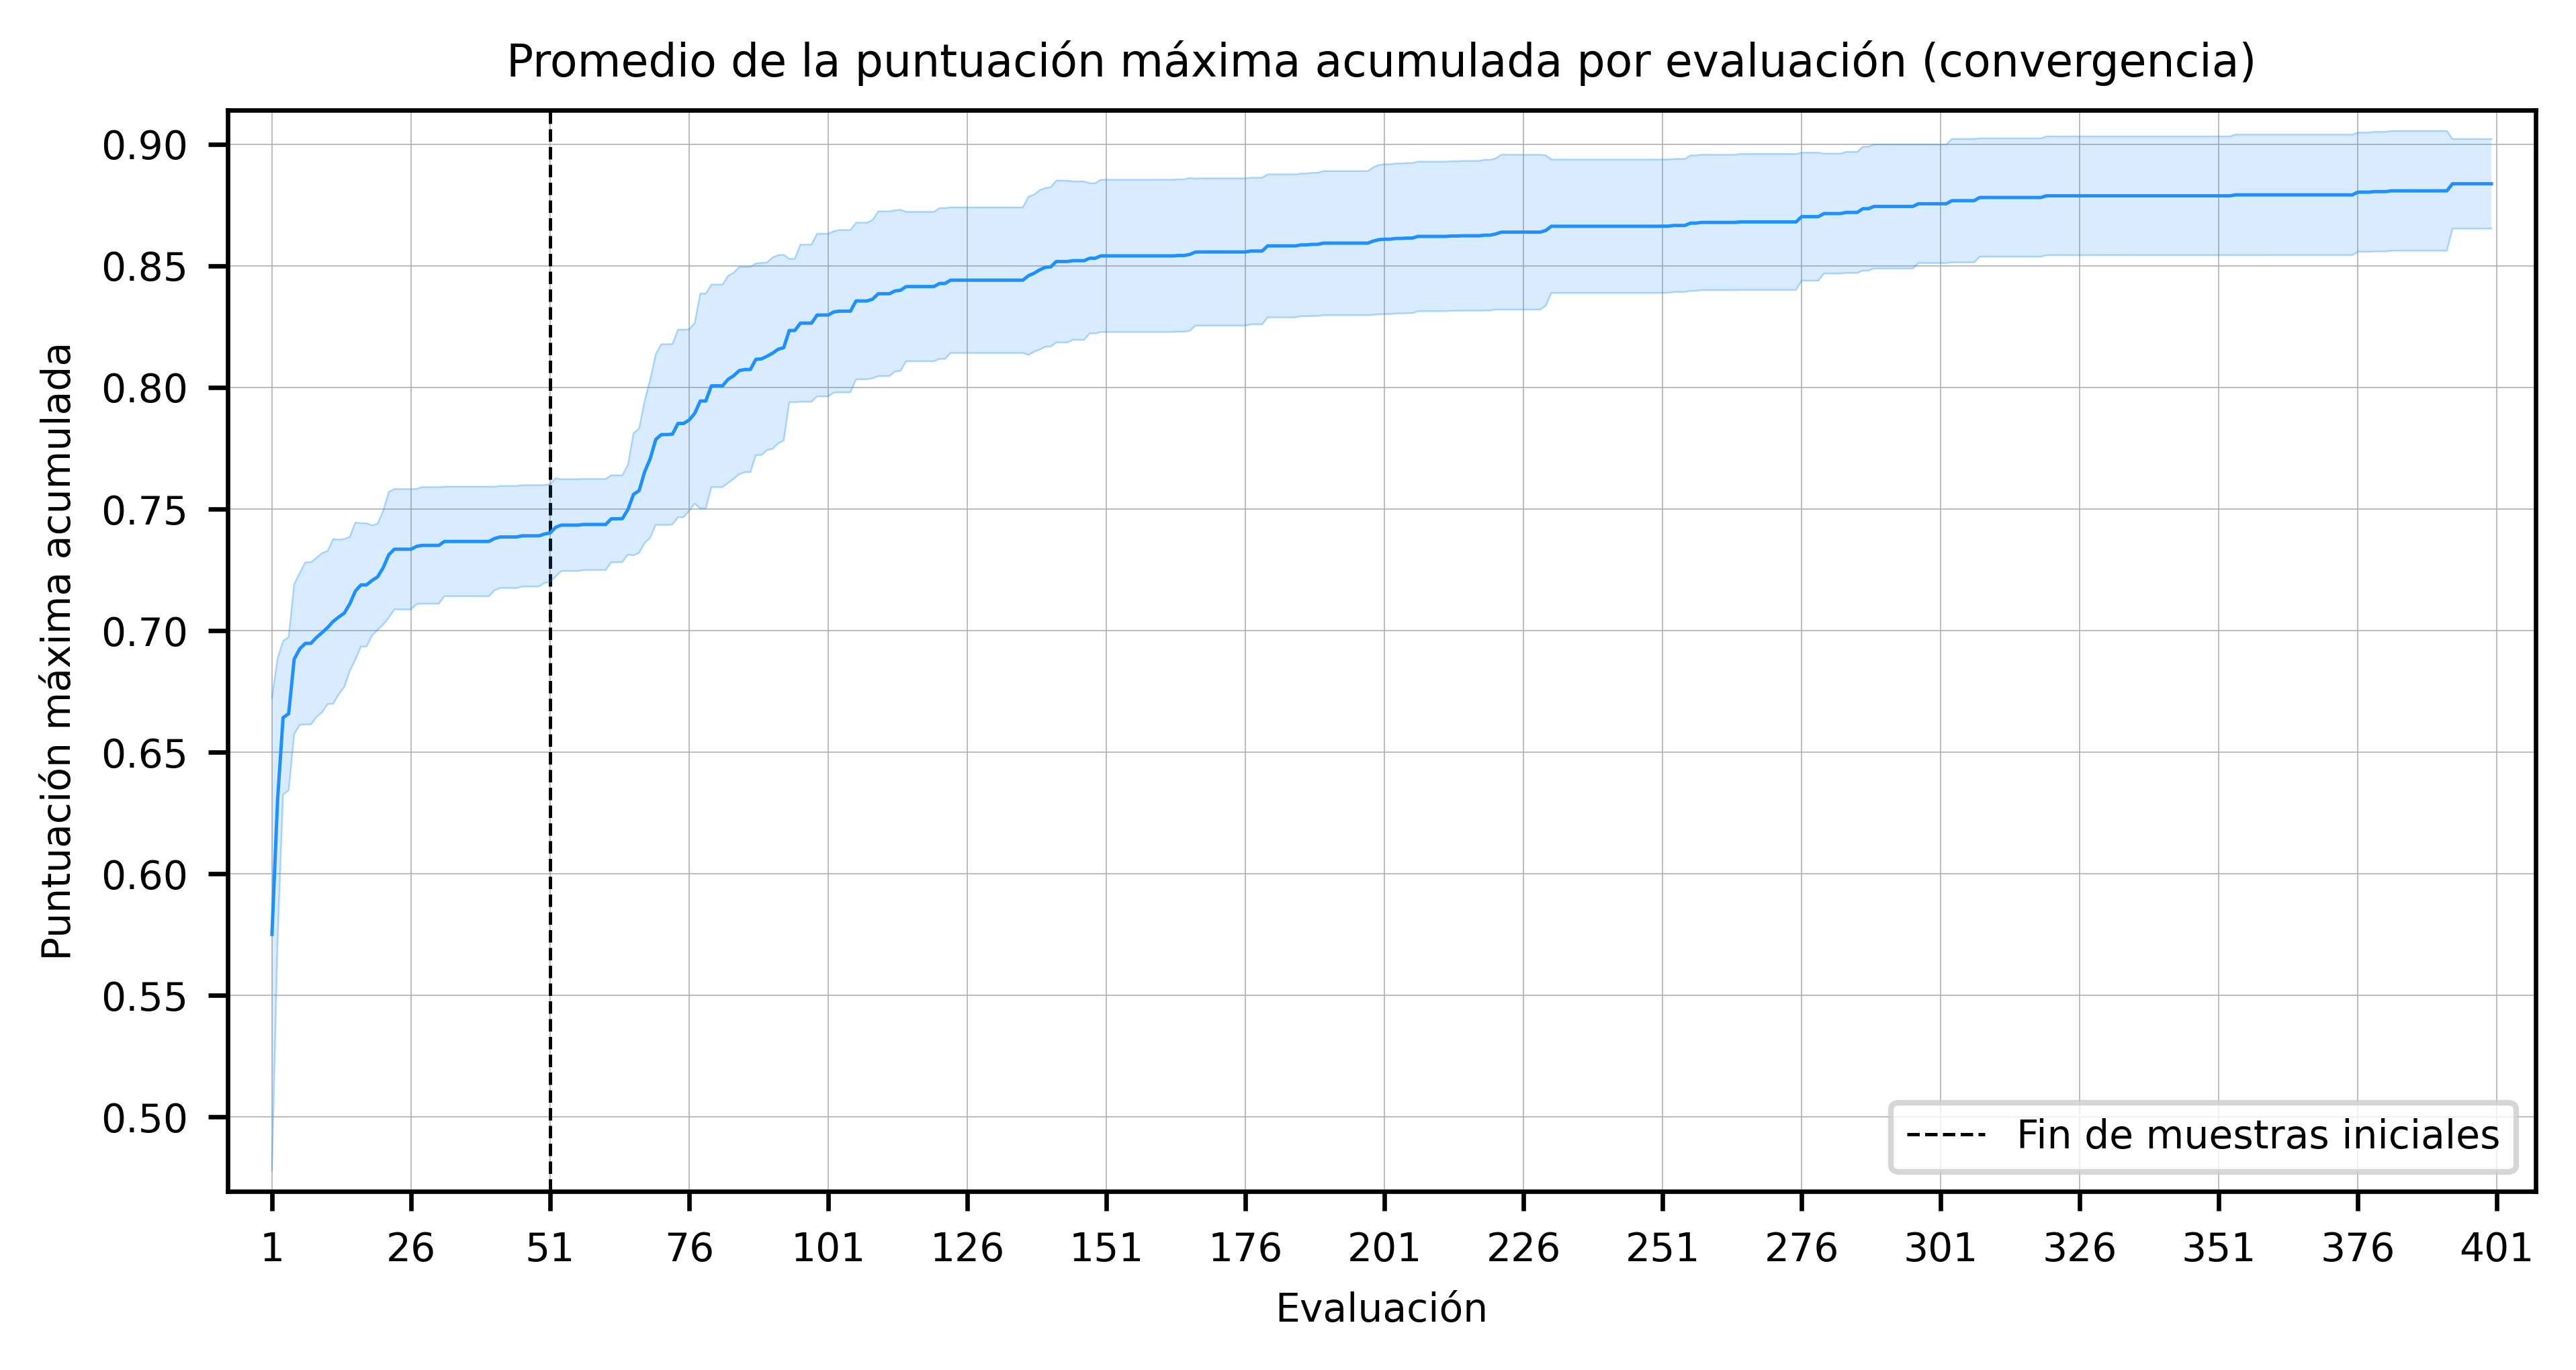
\includegraphics[width=\textwidth, height=\textheight, keepaspectratio]{bo_history_offline_syn_i_antiphase_acc_max}
    \vfill
\end{frame}


\begin{frame}{Convergencia de la implementación \textit{offline}: fase}
    \vfill
    \centering
    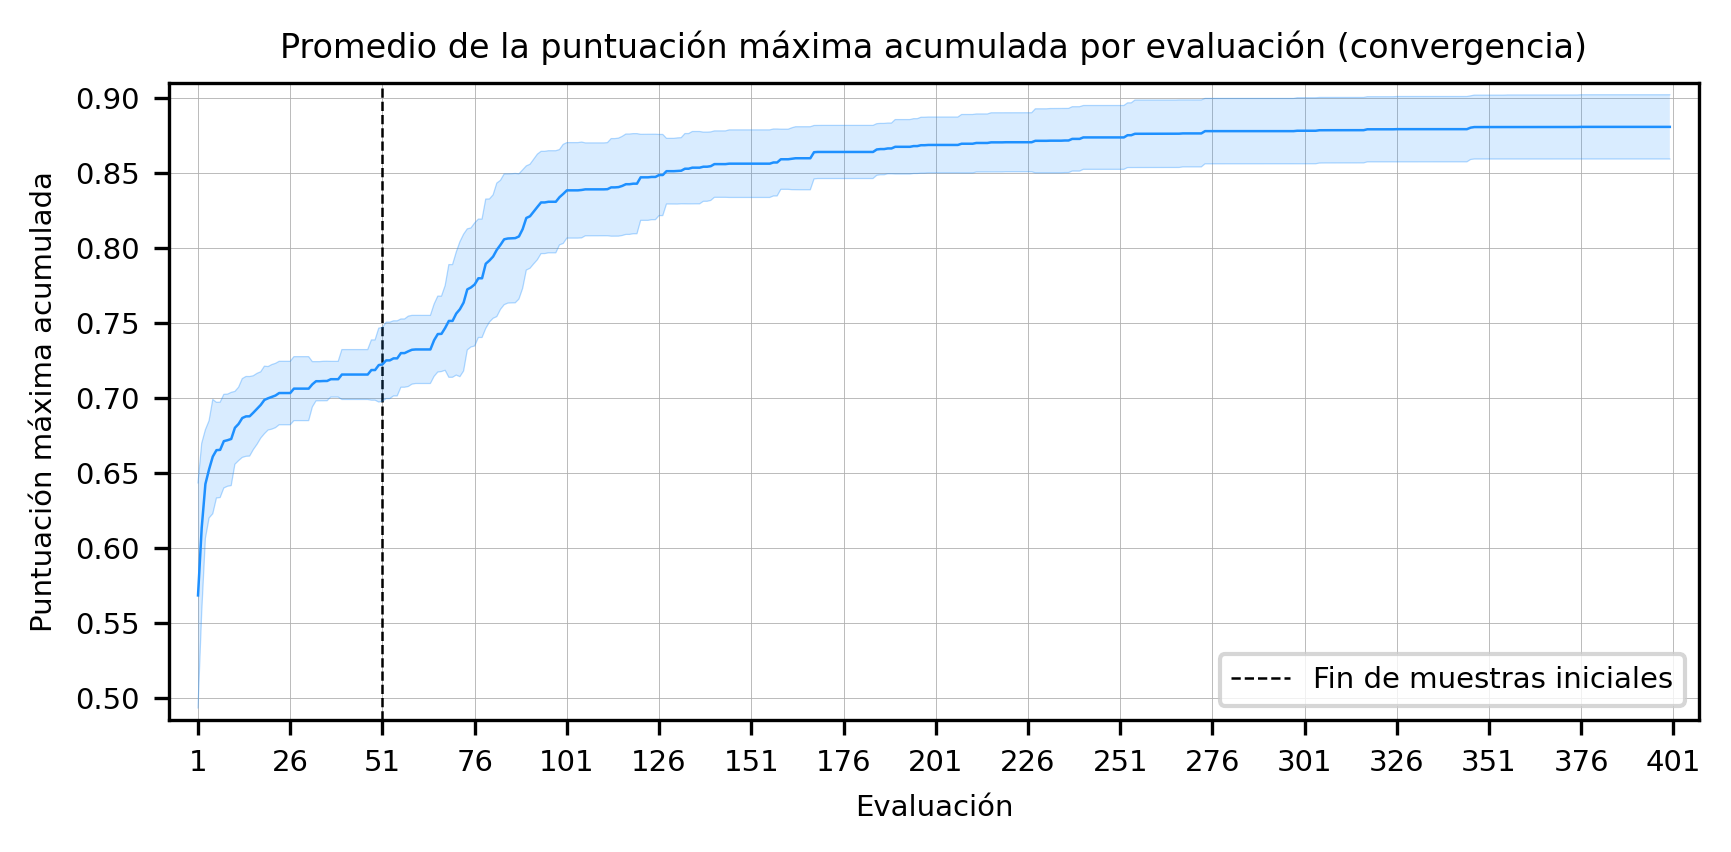
\includegraphics[width=\textwidth, height=\textheight, keepaspectratio]{bo_history_offline_syn_i_phase_acc_max}
    \vfill
\end{frame}


\begin{frame}{Puntuaciones de la implementación \textit{offline}: fase: antifase}
    \vfill
    \centering
    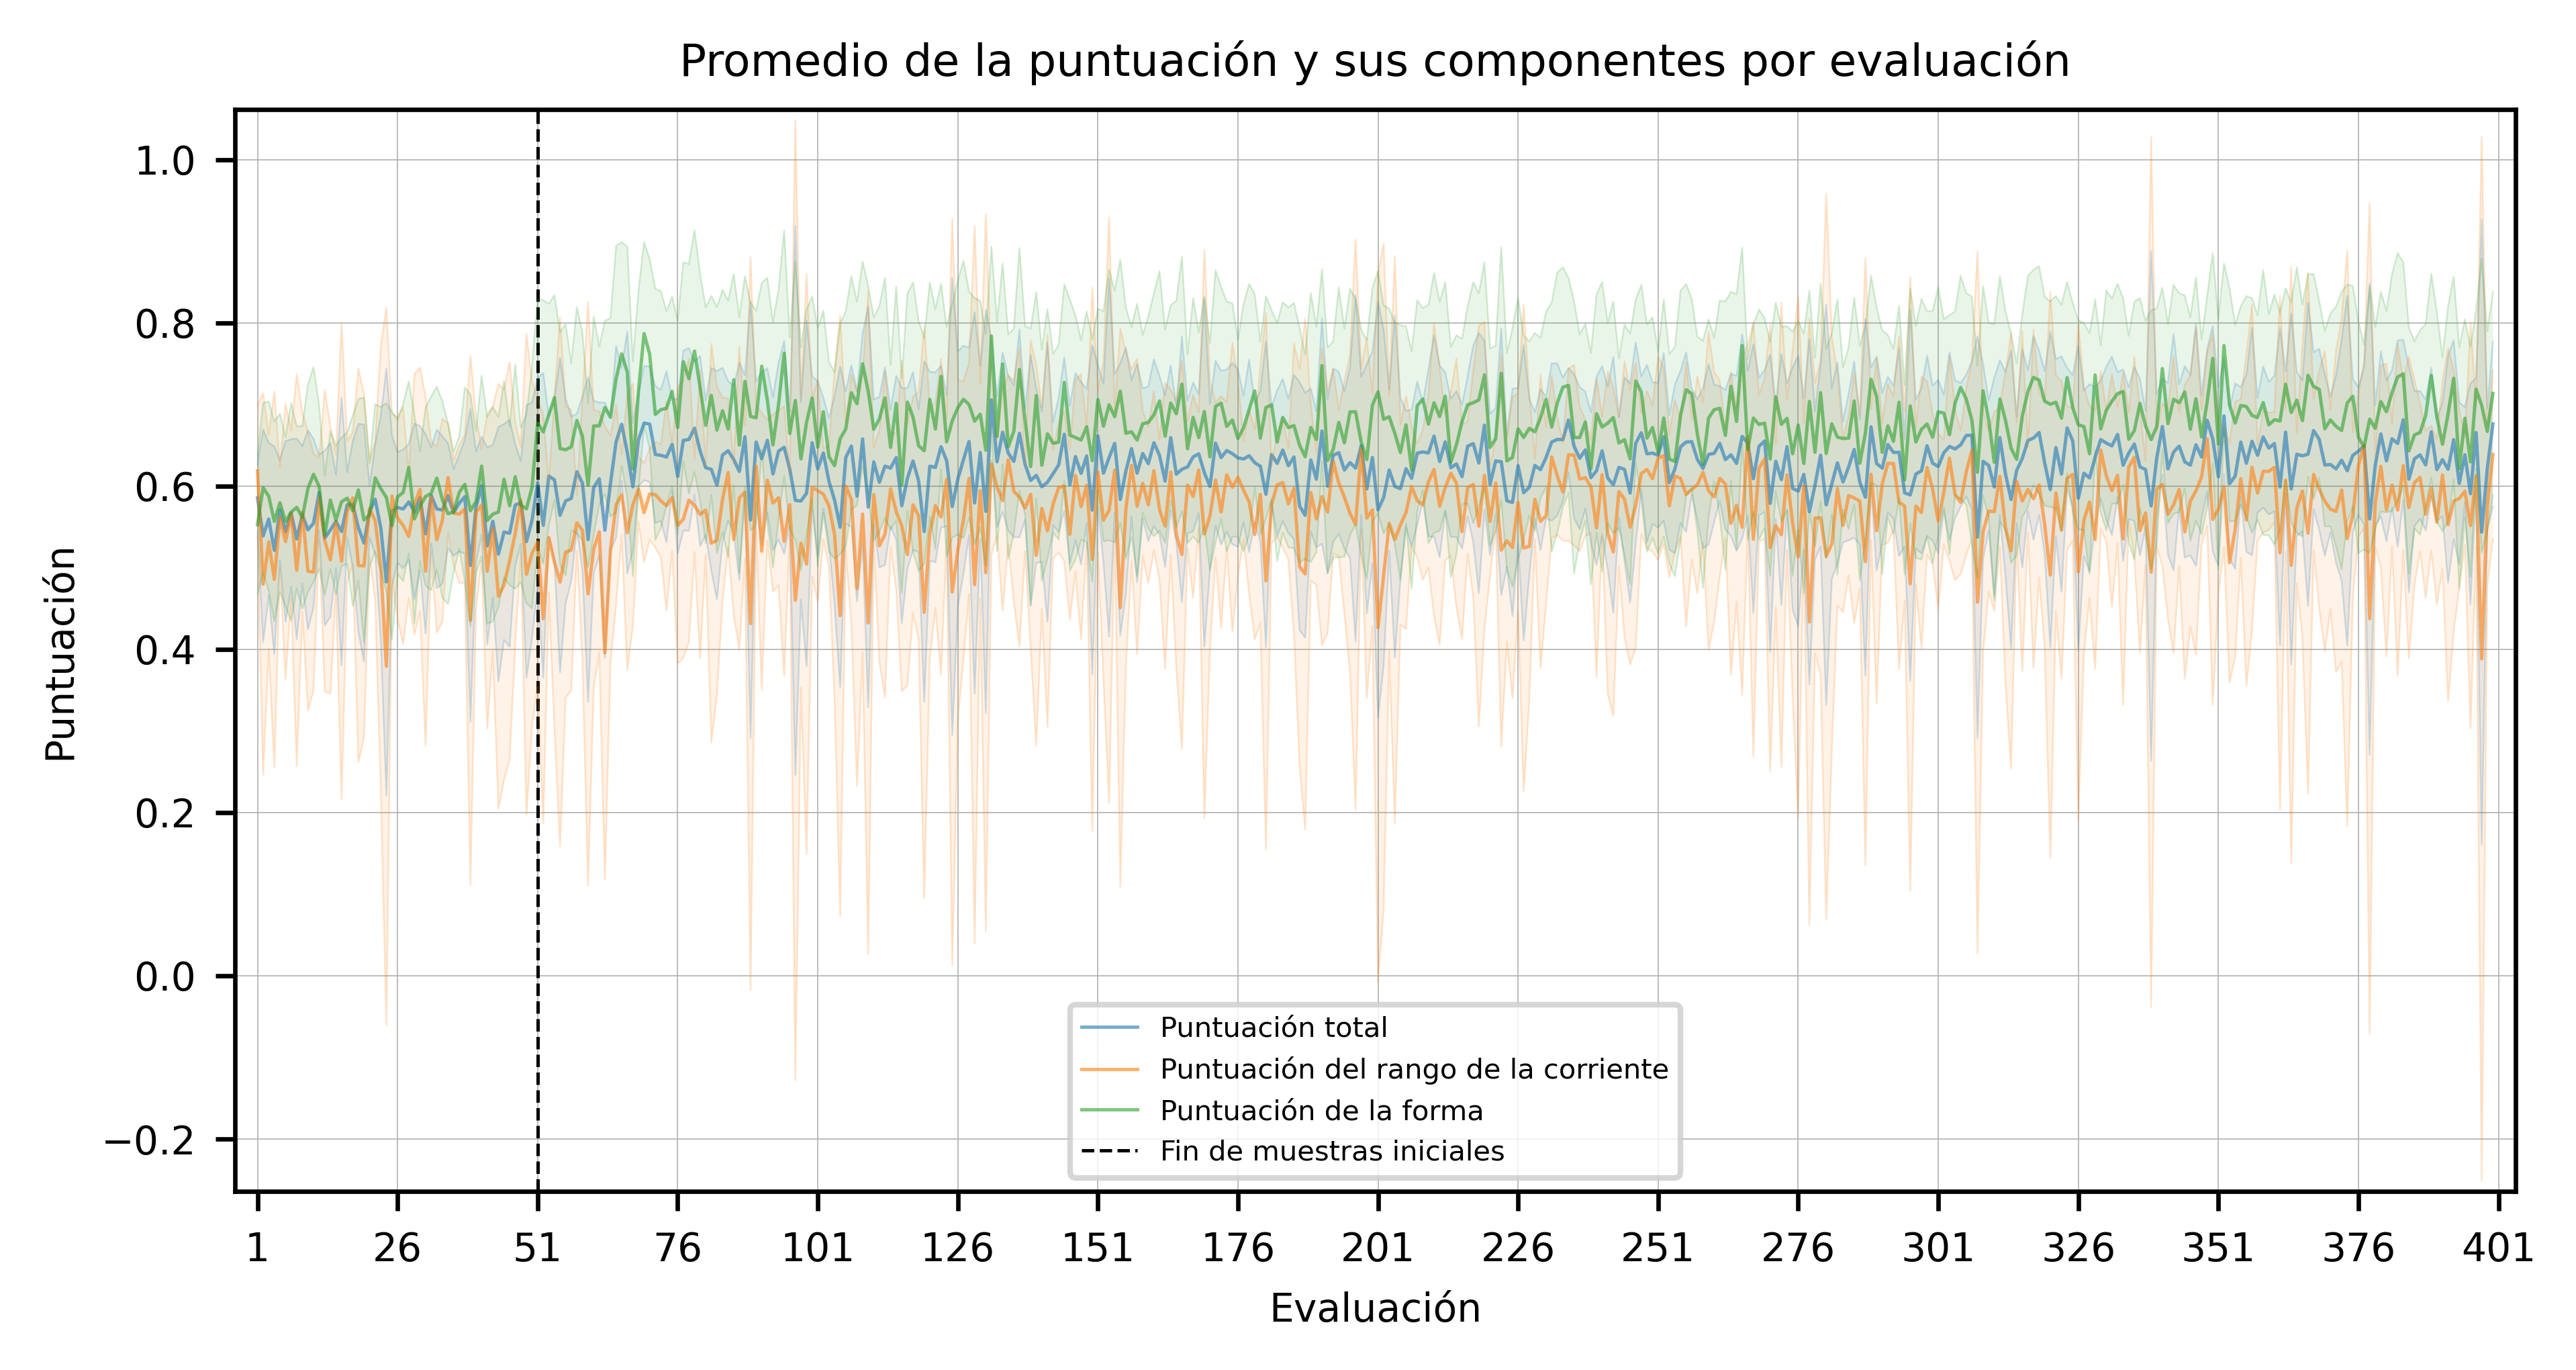
\includegraphics[width=\textwidth, height=\textheight, keepaspectratio]{bo_history_offline_syn_i_antiphase_avg_scores}
    \vfill
\end{frame}


\begin{frame}{Puntuaciones de una ejecución de la implementación \textit{offline}: antifase}
    \vfill
    \centering
    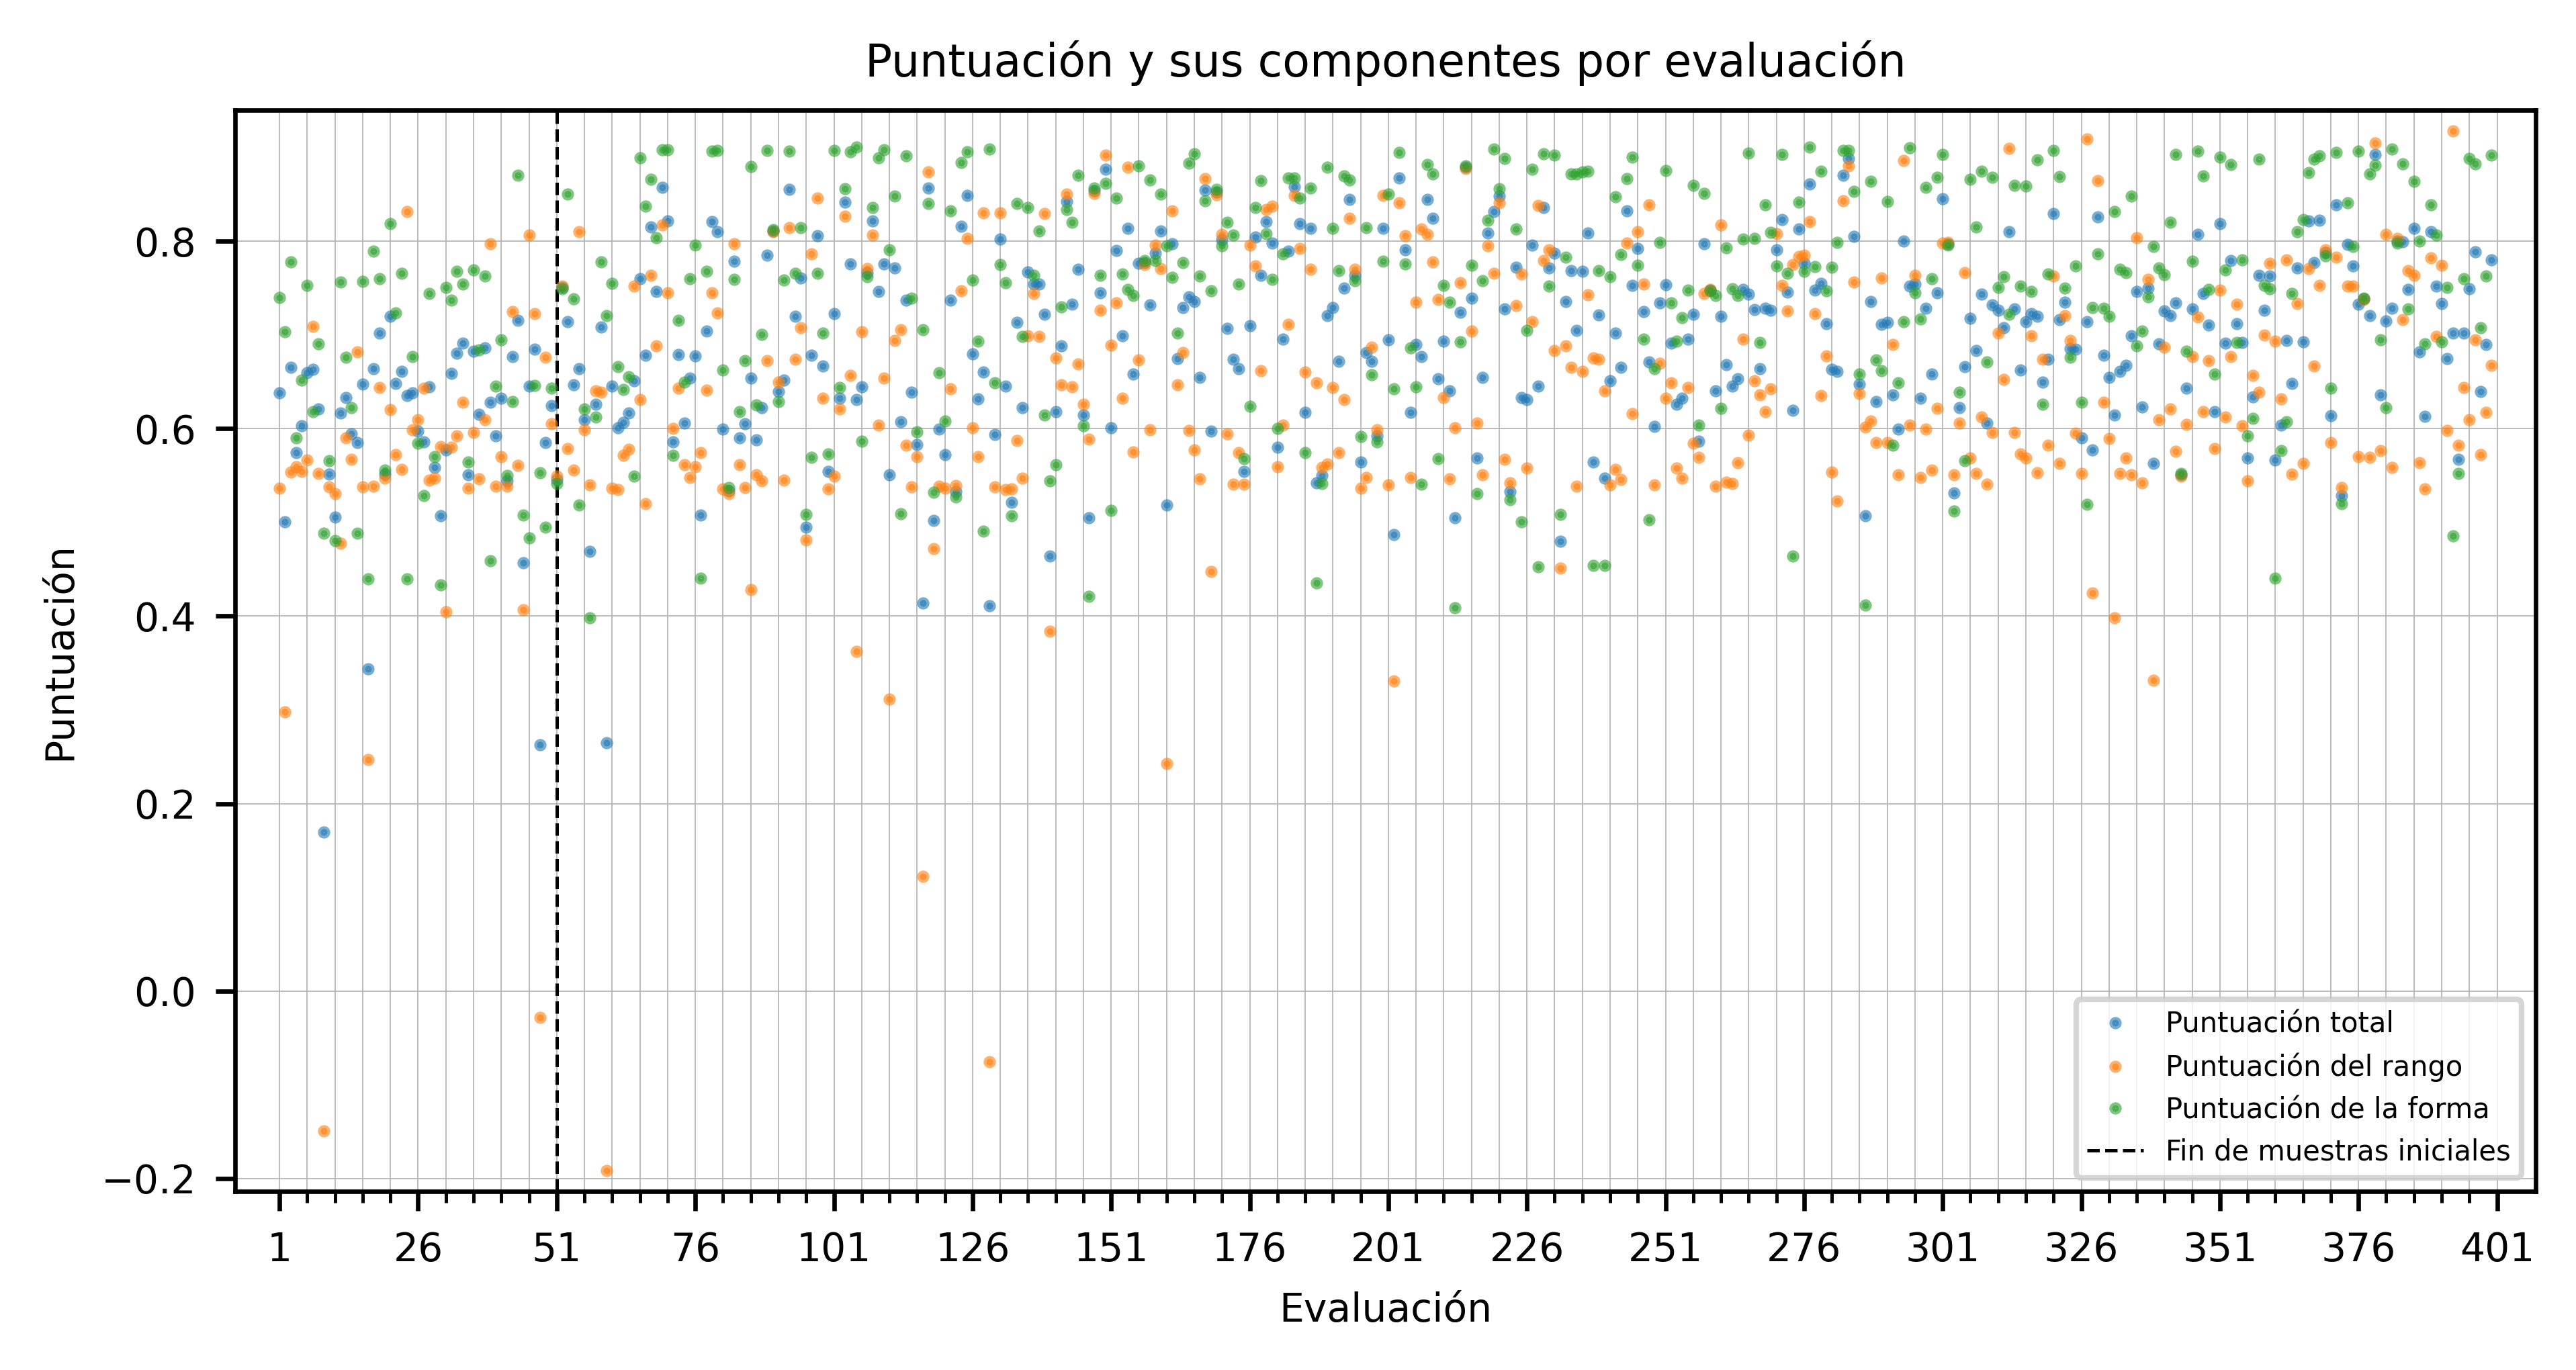
\includegraphics[width=\textwidth, height=\textheight, keepaspectratio]{bo_history_offline_syn_i_antiphase_scores}
    \vfill
\end{frame}


\begin{frame}{Dinámica resultante de la implementación \textit{offline}: antifase}
    \vfill
    \centering
    \vspace{-0.3em}
    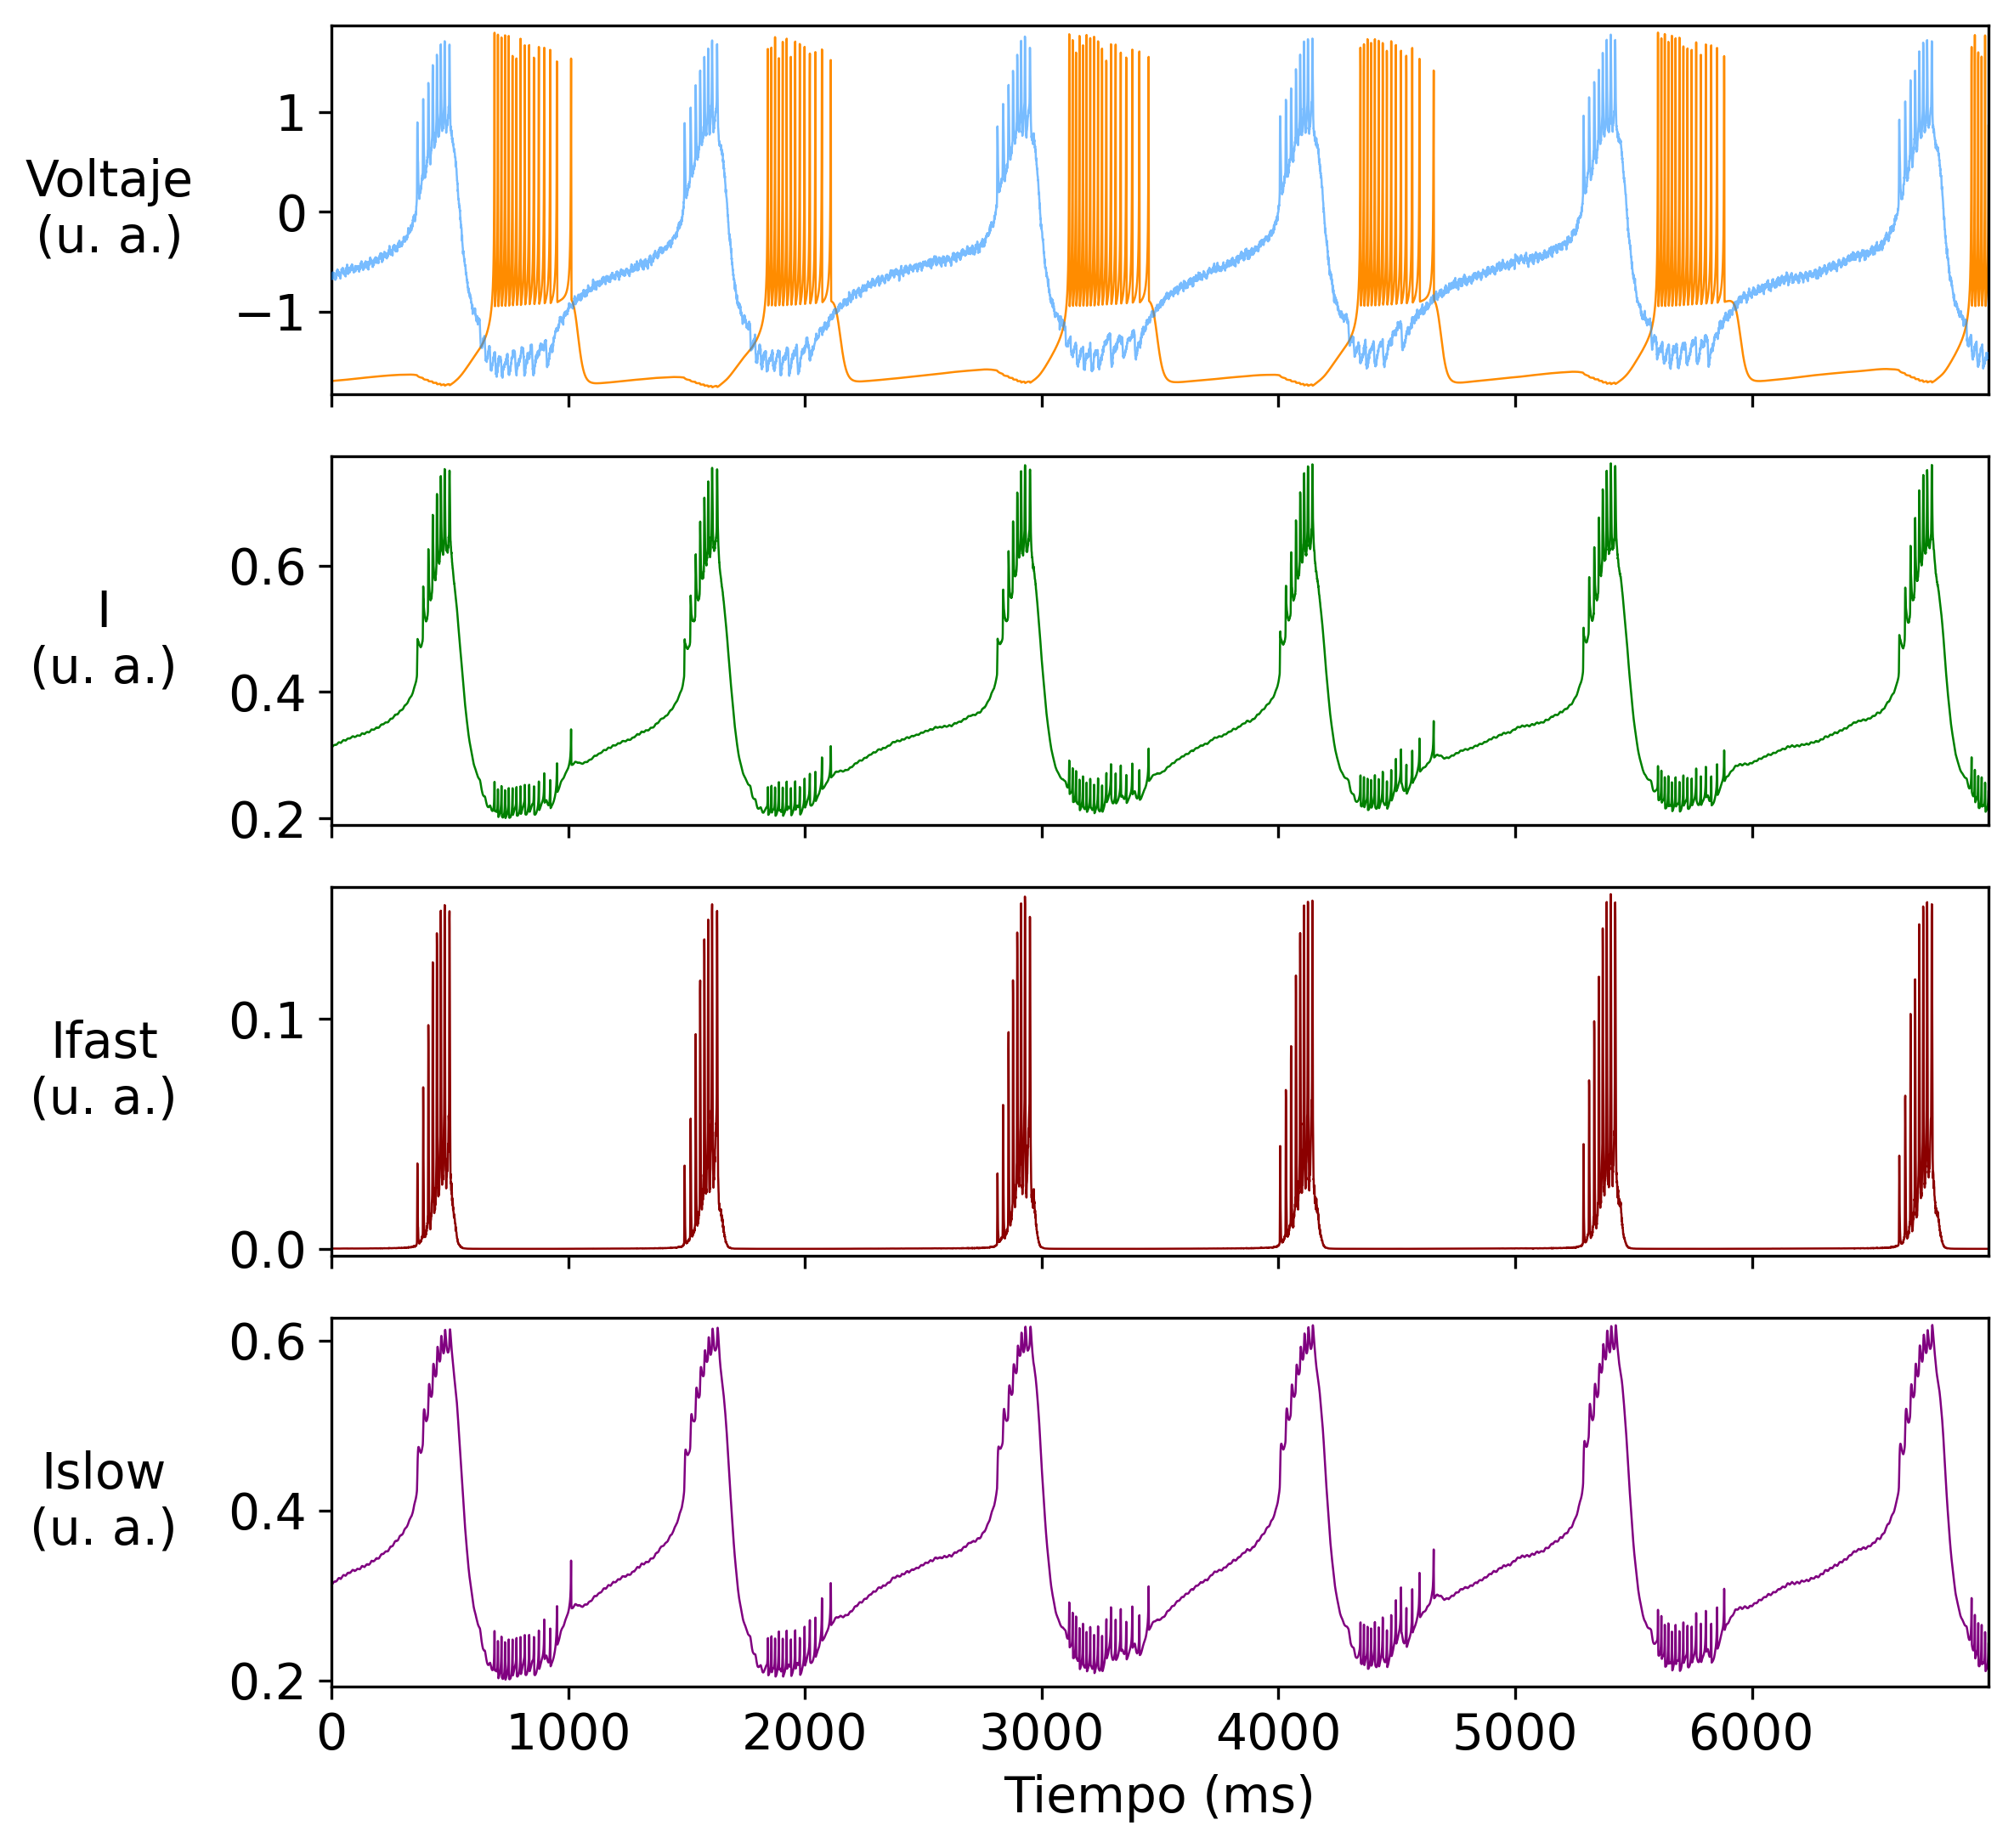
\includegraphics[height=0.88\textheight, keepaspectratio]{offline_syn_i_antiphase}
    \vfill
\end{frame}


\begin{frame}{Dinámica resultante de la implementación \textit{offline}: fase}
    \vfill
    \centering
    \vspace{-0.3em}
    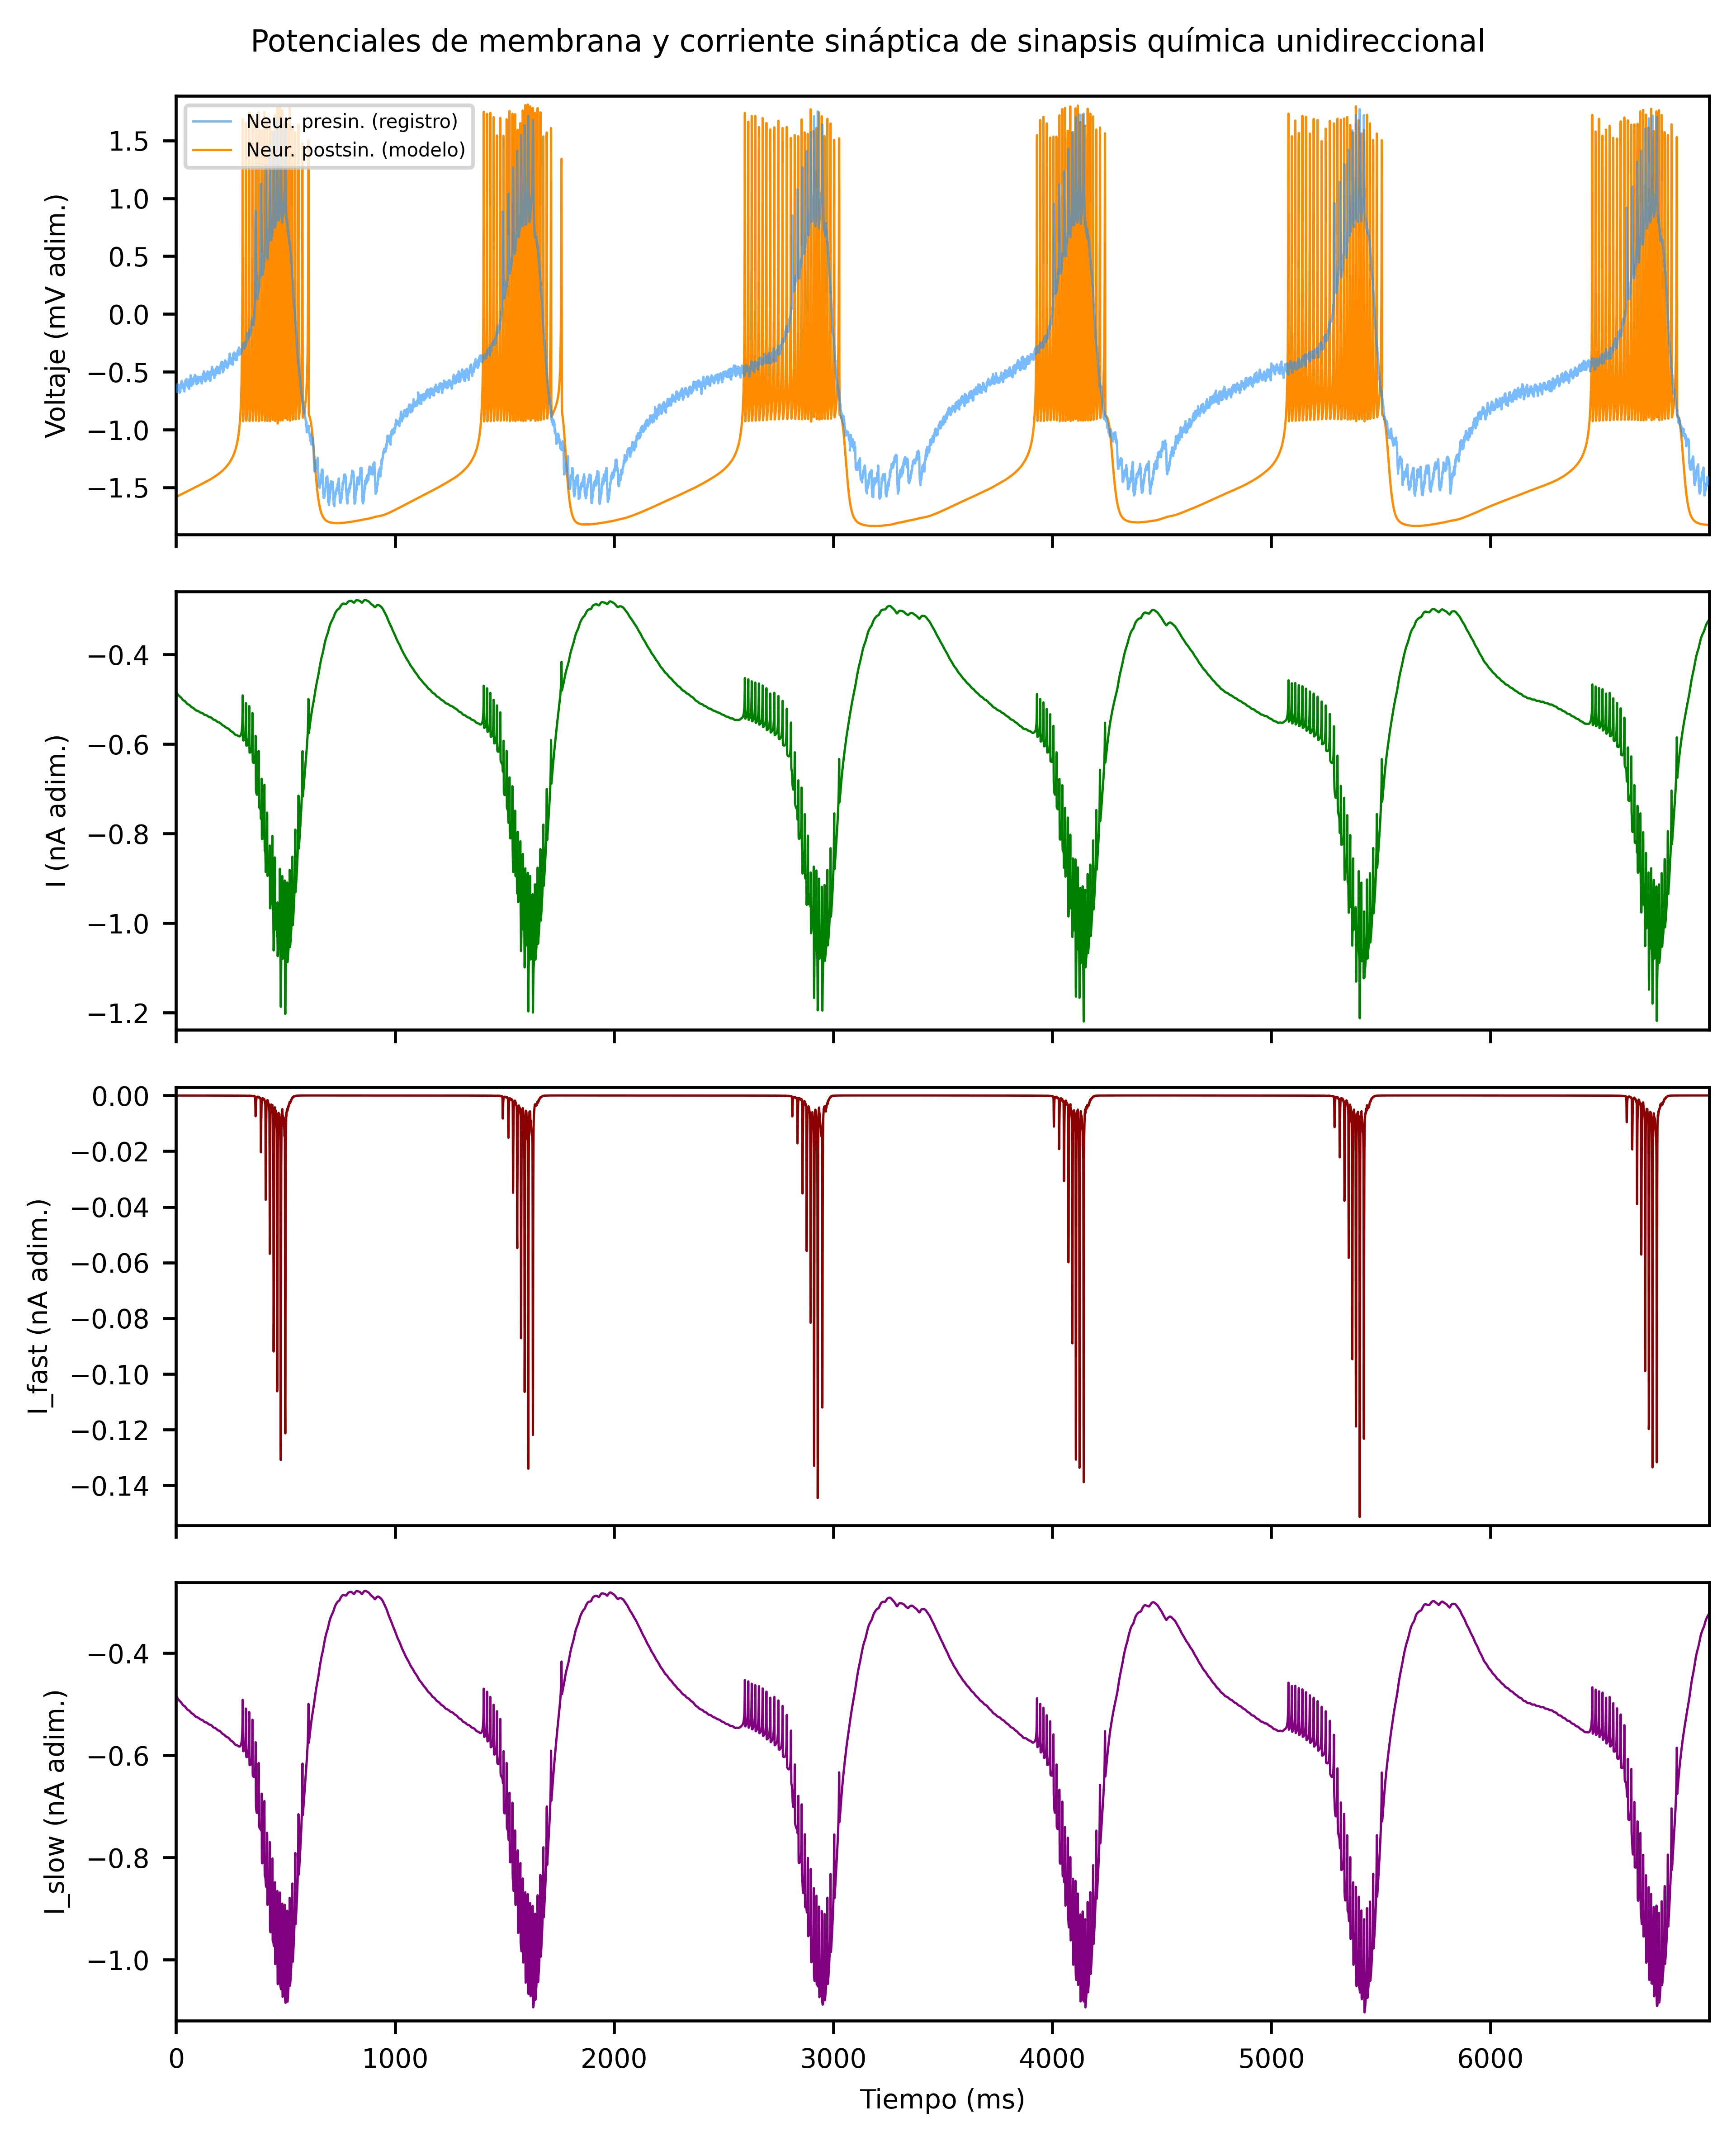
\includegraphics[height=0.88\textheight, keepaspectratio]{offline_syn_i_phase}
    \vfill
\end{frame}


\begin{frame}{Resultados de la implementación \textit{online}}
    \scriptsize
    \begin{columns}[t]
        \begin{column}{0.48\textwidth}
            Configuraciones:
            \begin{itemize}
                \item $\boldsymbol{I_{\mathrm{fast}}}$ en un sentido e $\boldsymbol{I_{\mathrm{slow}}}$ en otro $\to$ dimensionalidad razonable (10).
                \item \textbf{Ambas neuronas modelo}, con periodo de \textit{burst} de $\boldsymbol{1{,}6}$\,\textbf{s}.
                \item Estabilización de $\boldsymbol{400}$\,\textbf{ms} y \textbf{evaluación} de $\boldsymbol{1800}$\,\textbf{ms} ($\boldsymbol{\sim 1}$ \textbf{periodo de \textit{burst}}). \textbf{Tiempo real}.
                \item Periodo de RTXI: $\boldsymbol{1}$\,\textbf{kHz}.
                \item Frecuencia de corte de $0{,}002$\,kHz (\textit{spikes} de la Hindmarsh-Rose anchos).
                \item \textbf{Sin promedios} por los altos tiempos.
                \item \textbf{Rangos de corriente objetivo}:
                      \begin{itemize}
                          \scriptsize
                          \item \textbf{Antifase}: $\boldsymbol{[-1{,}0; -0{,}0]}$ u. a. para $\boldsymbol{I_{\mathrm{fast}}}$, $\boldsymbol{[-1{,}4; -0{,}4]}$ u. a. para $\boldsymbol{I_{\mathrm{slow}}}$.
                          \item \textbf{Fase}: $\boldsymbol{[0{,}0; 0{,}6]}$ u. a. para $\boldsymbol{I_{\mathrm{fast}}}$, $\boldsymbol{[0{,}2; 0{,}8]}$ u. a. para $\boldsymbol{I_{\mathrm{slow}}}$.
                      \end{itemize}
            \end{itemize}
        \end{column}
        \begin{column}{0.48\textwidth}
            Tiempos obtenidos:
            \begin{itemize}
                \item \textbf{Antifase}: $\boldsymbol{915{,}46}$\,\textbf{s} ($\boldsymbol{\sim 15}$ \textbf{min.}).
                \item \textbf{Fase}: $\boldsymbol{934{,}14}$\,\textbf{s} ($\boldsymbol{\sim 16}$ \textbf{min.}).
            \end{itemize}
        \end{column}
    \end{columns}
\end{frame}


\begin{frame}{Convergencia de la implementación \textit{online}: antifase}
    \vfill
    \centering
    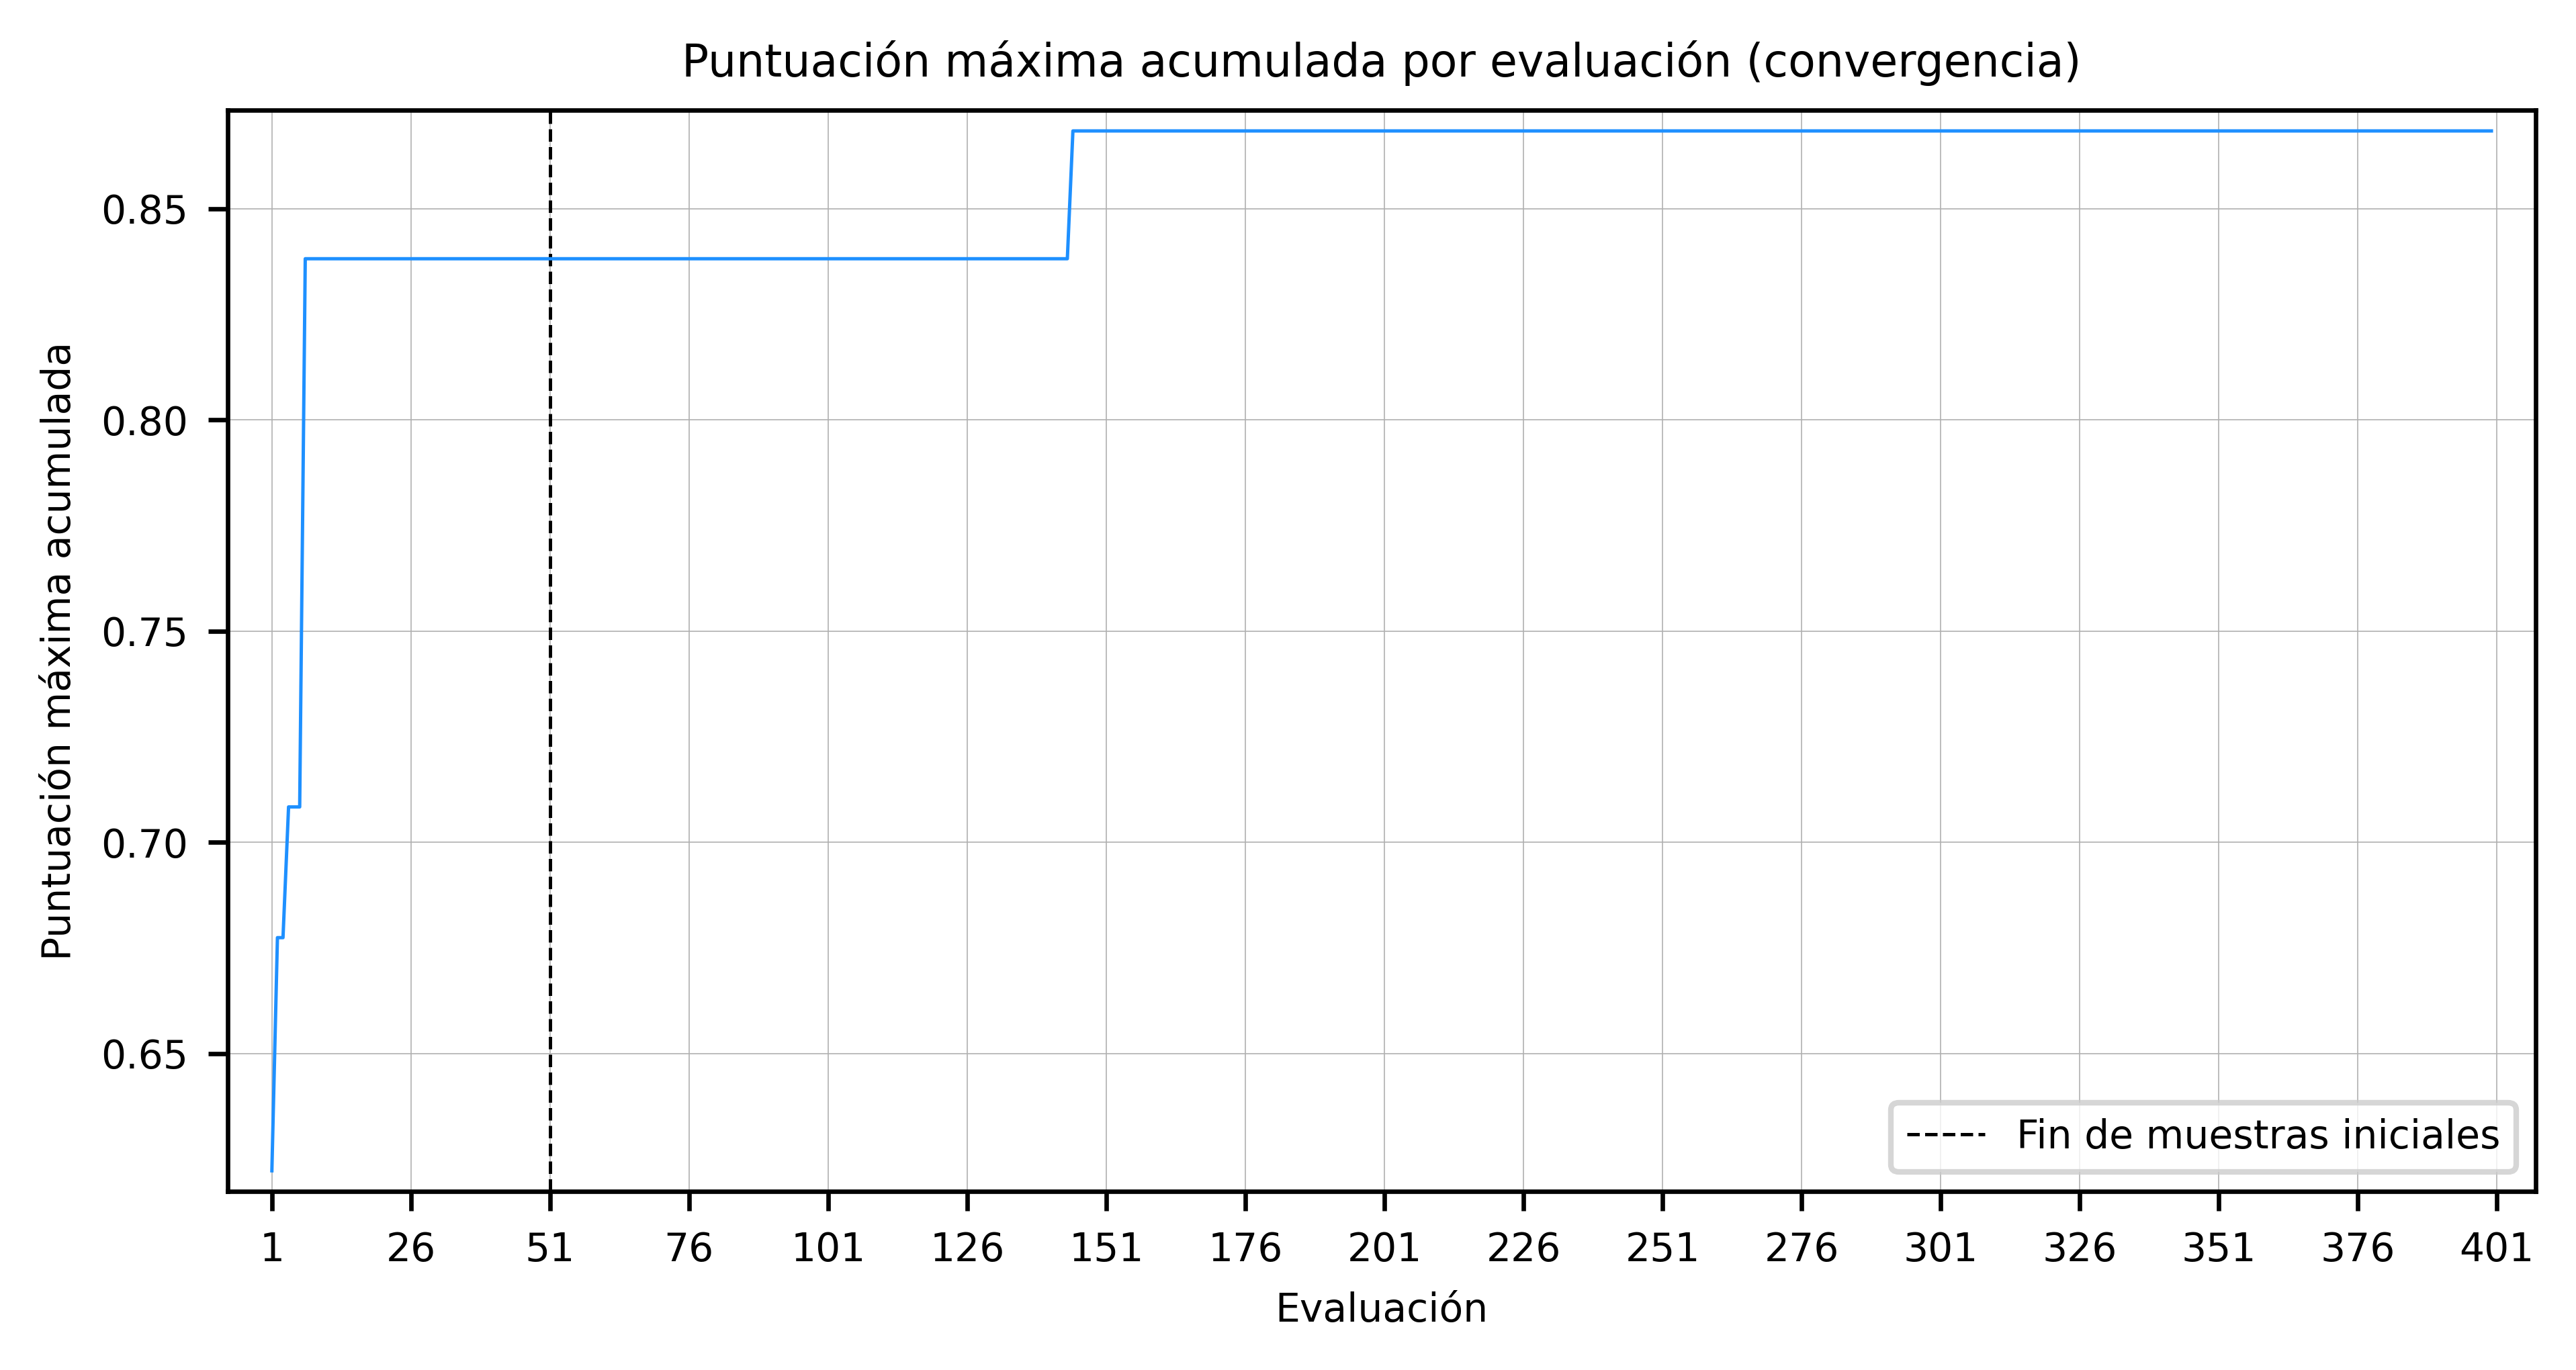
\includegraphics[width=\textwidth, height=\textheight, keepaspectratio]{bo_history_rtxi_syn_model_ifast_islow_antiphase_acc_max}
    \vfill
\end{frame}


\begin{frame}{Convergencia de la implementación \textit{online}: fase}
    \vfill
    \centering
    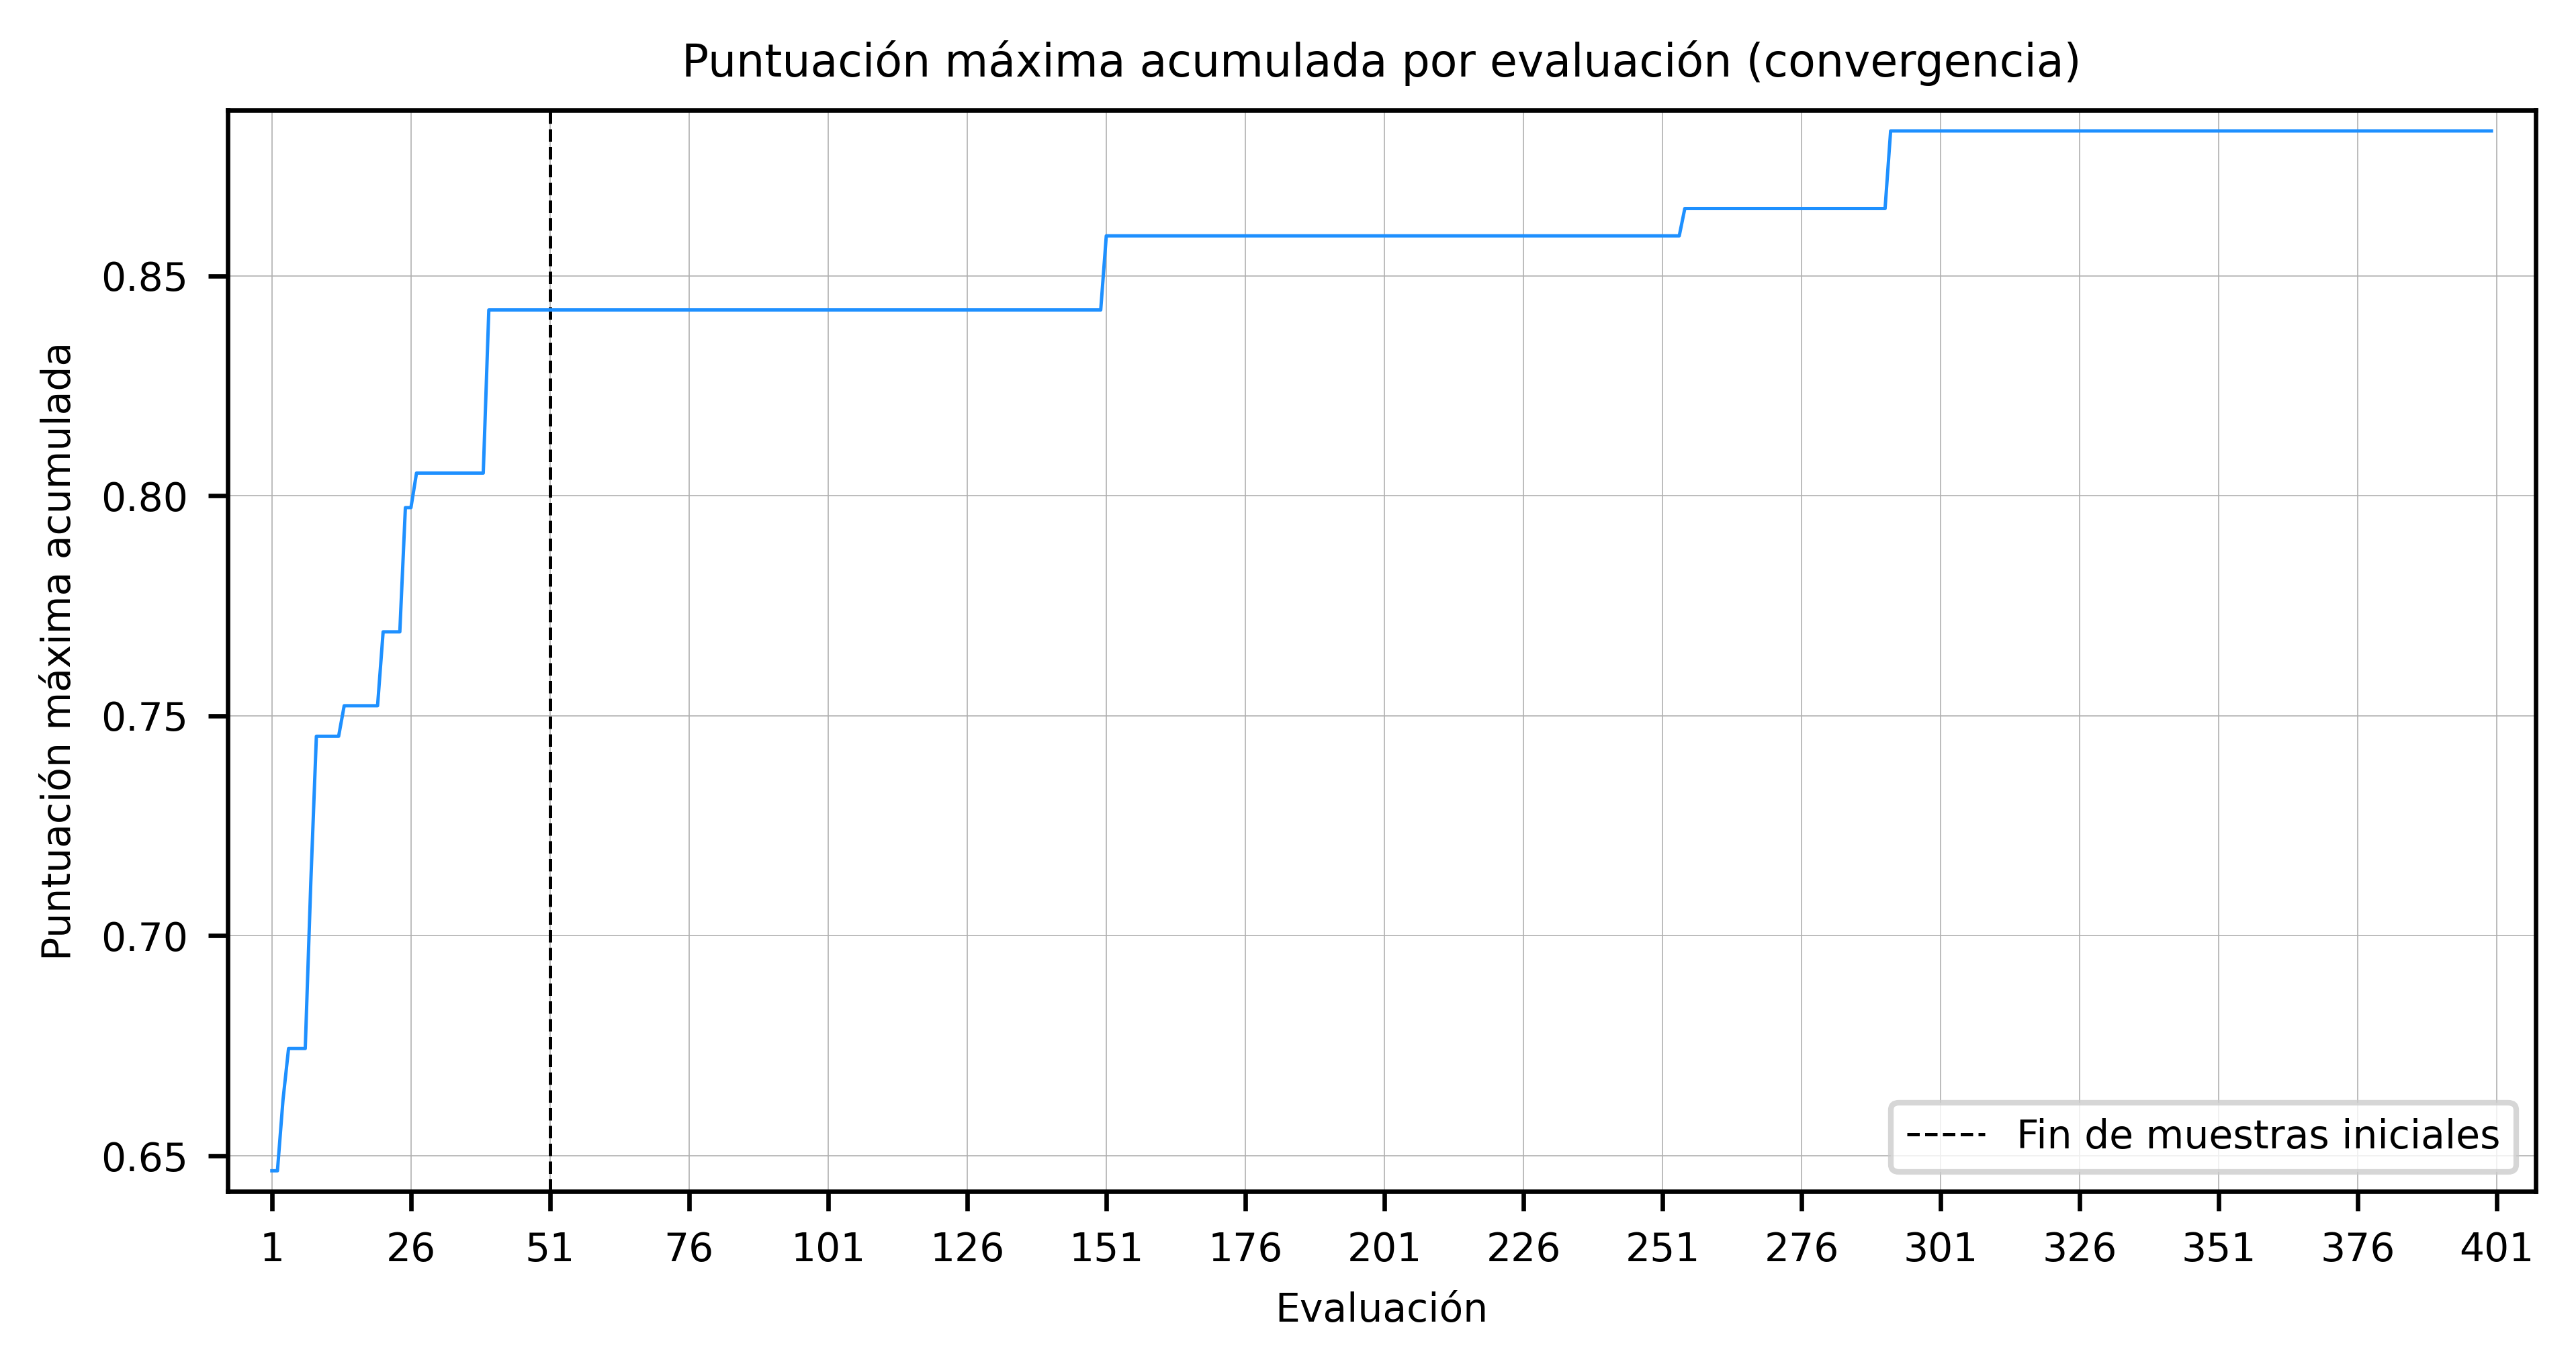
\includegraphics[width=\textwidth, height=\textheight, keepaspectratio]{bo_history_rtxi_syn_model_ifast_islow_phase_acc_max}
    \vfill
\end{frame}


\begin{frame}{Dinámica resultante de la implementación \textit{online}: antifase}
    \vfill
    \centering
    \vspace{-0.3em}
    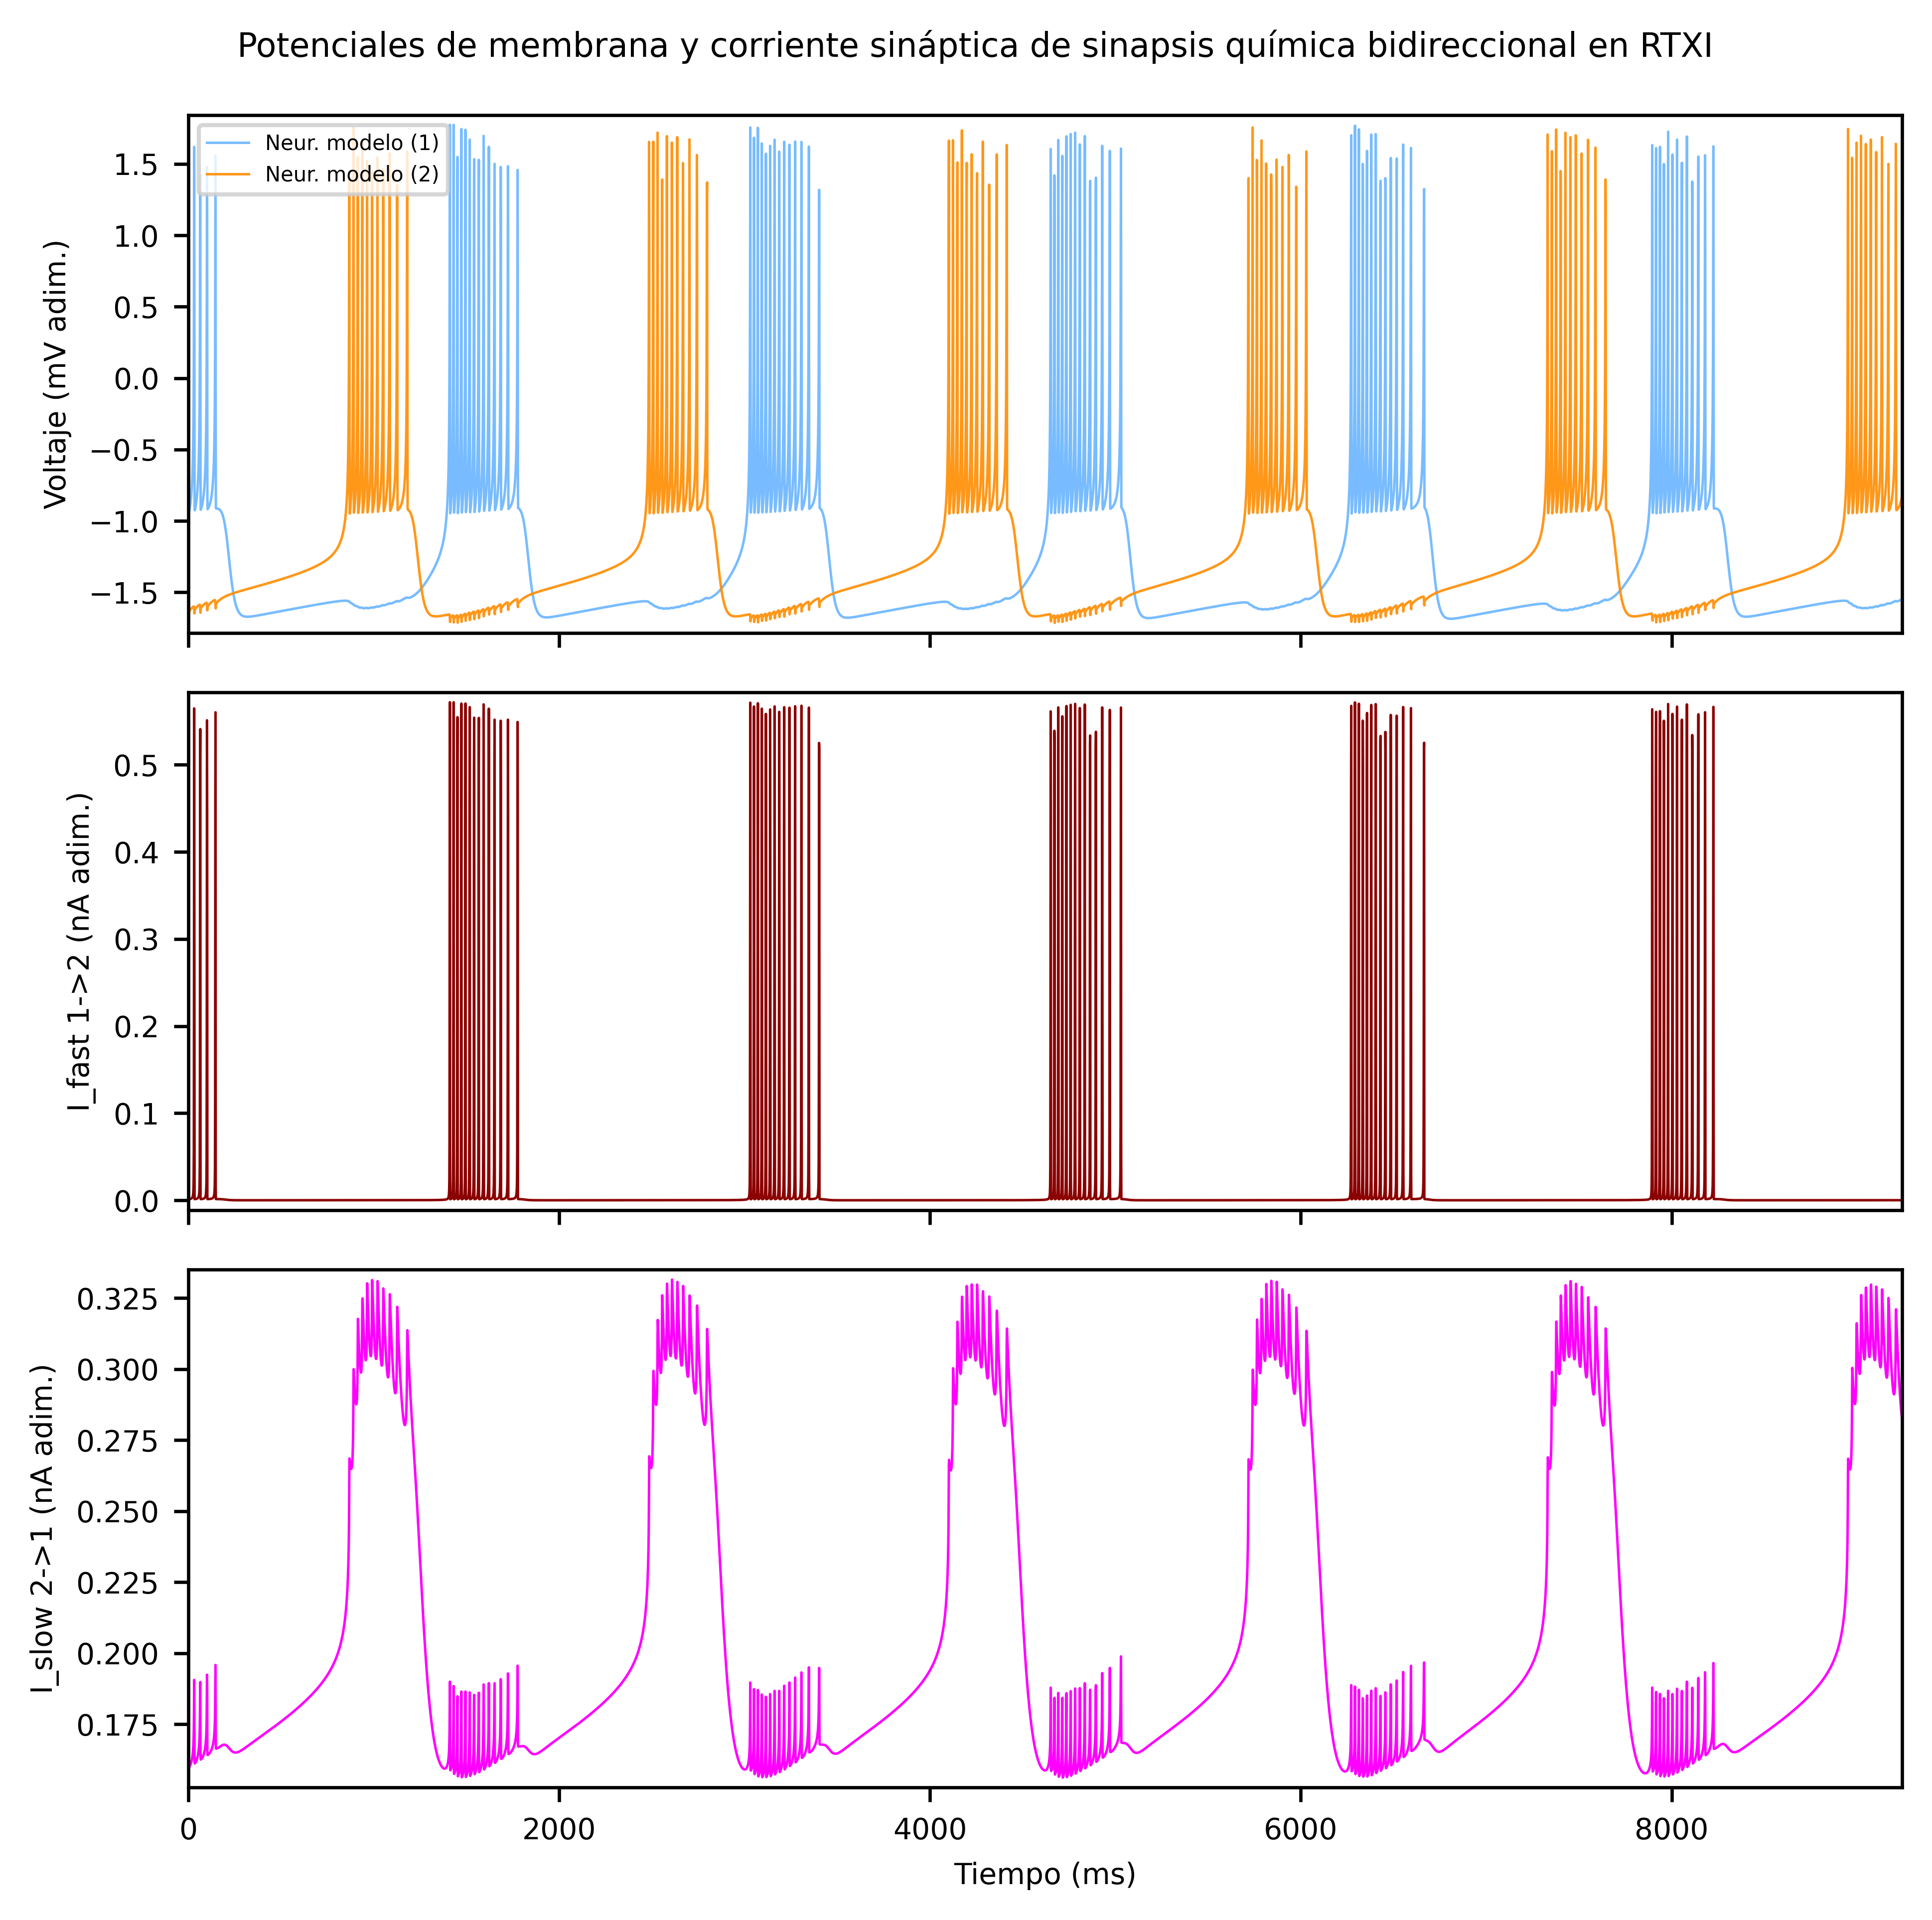
\includegraphics[width=\textwidth, height=0.88\textheight, keepaspectratio]{rtxi_syn_model_ifast_islow_antiphase}
    \vfill
\end{frame}


\begin{frame}{Dinámica resultante de la implementación \textit{online}: fase}
    \vfill
    \centering
    \vspace{-0.3em}
    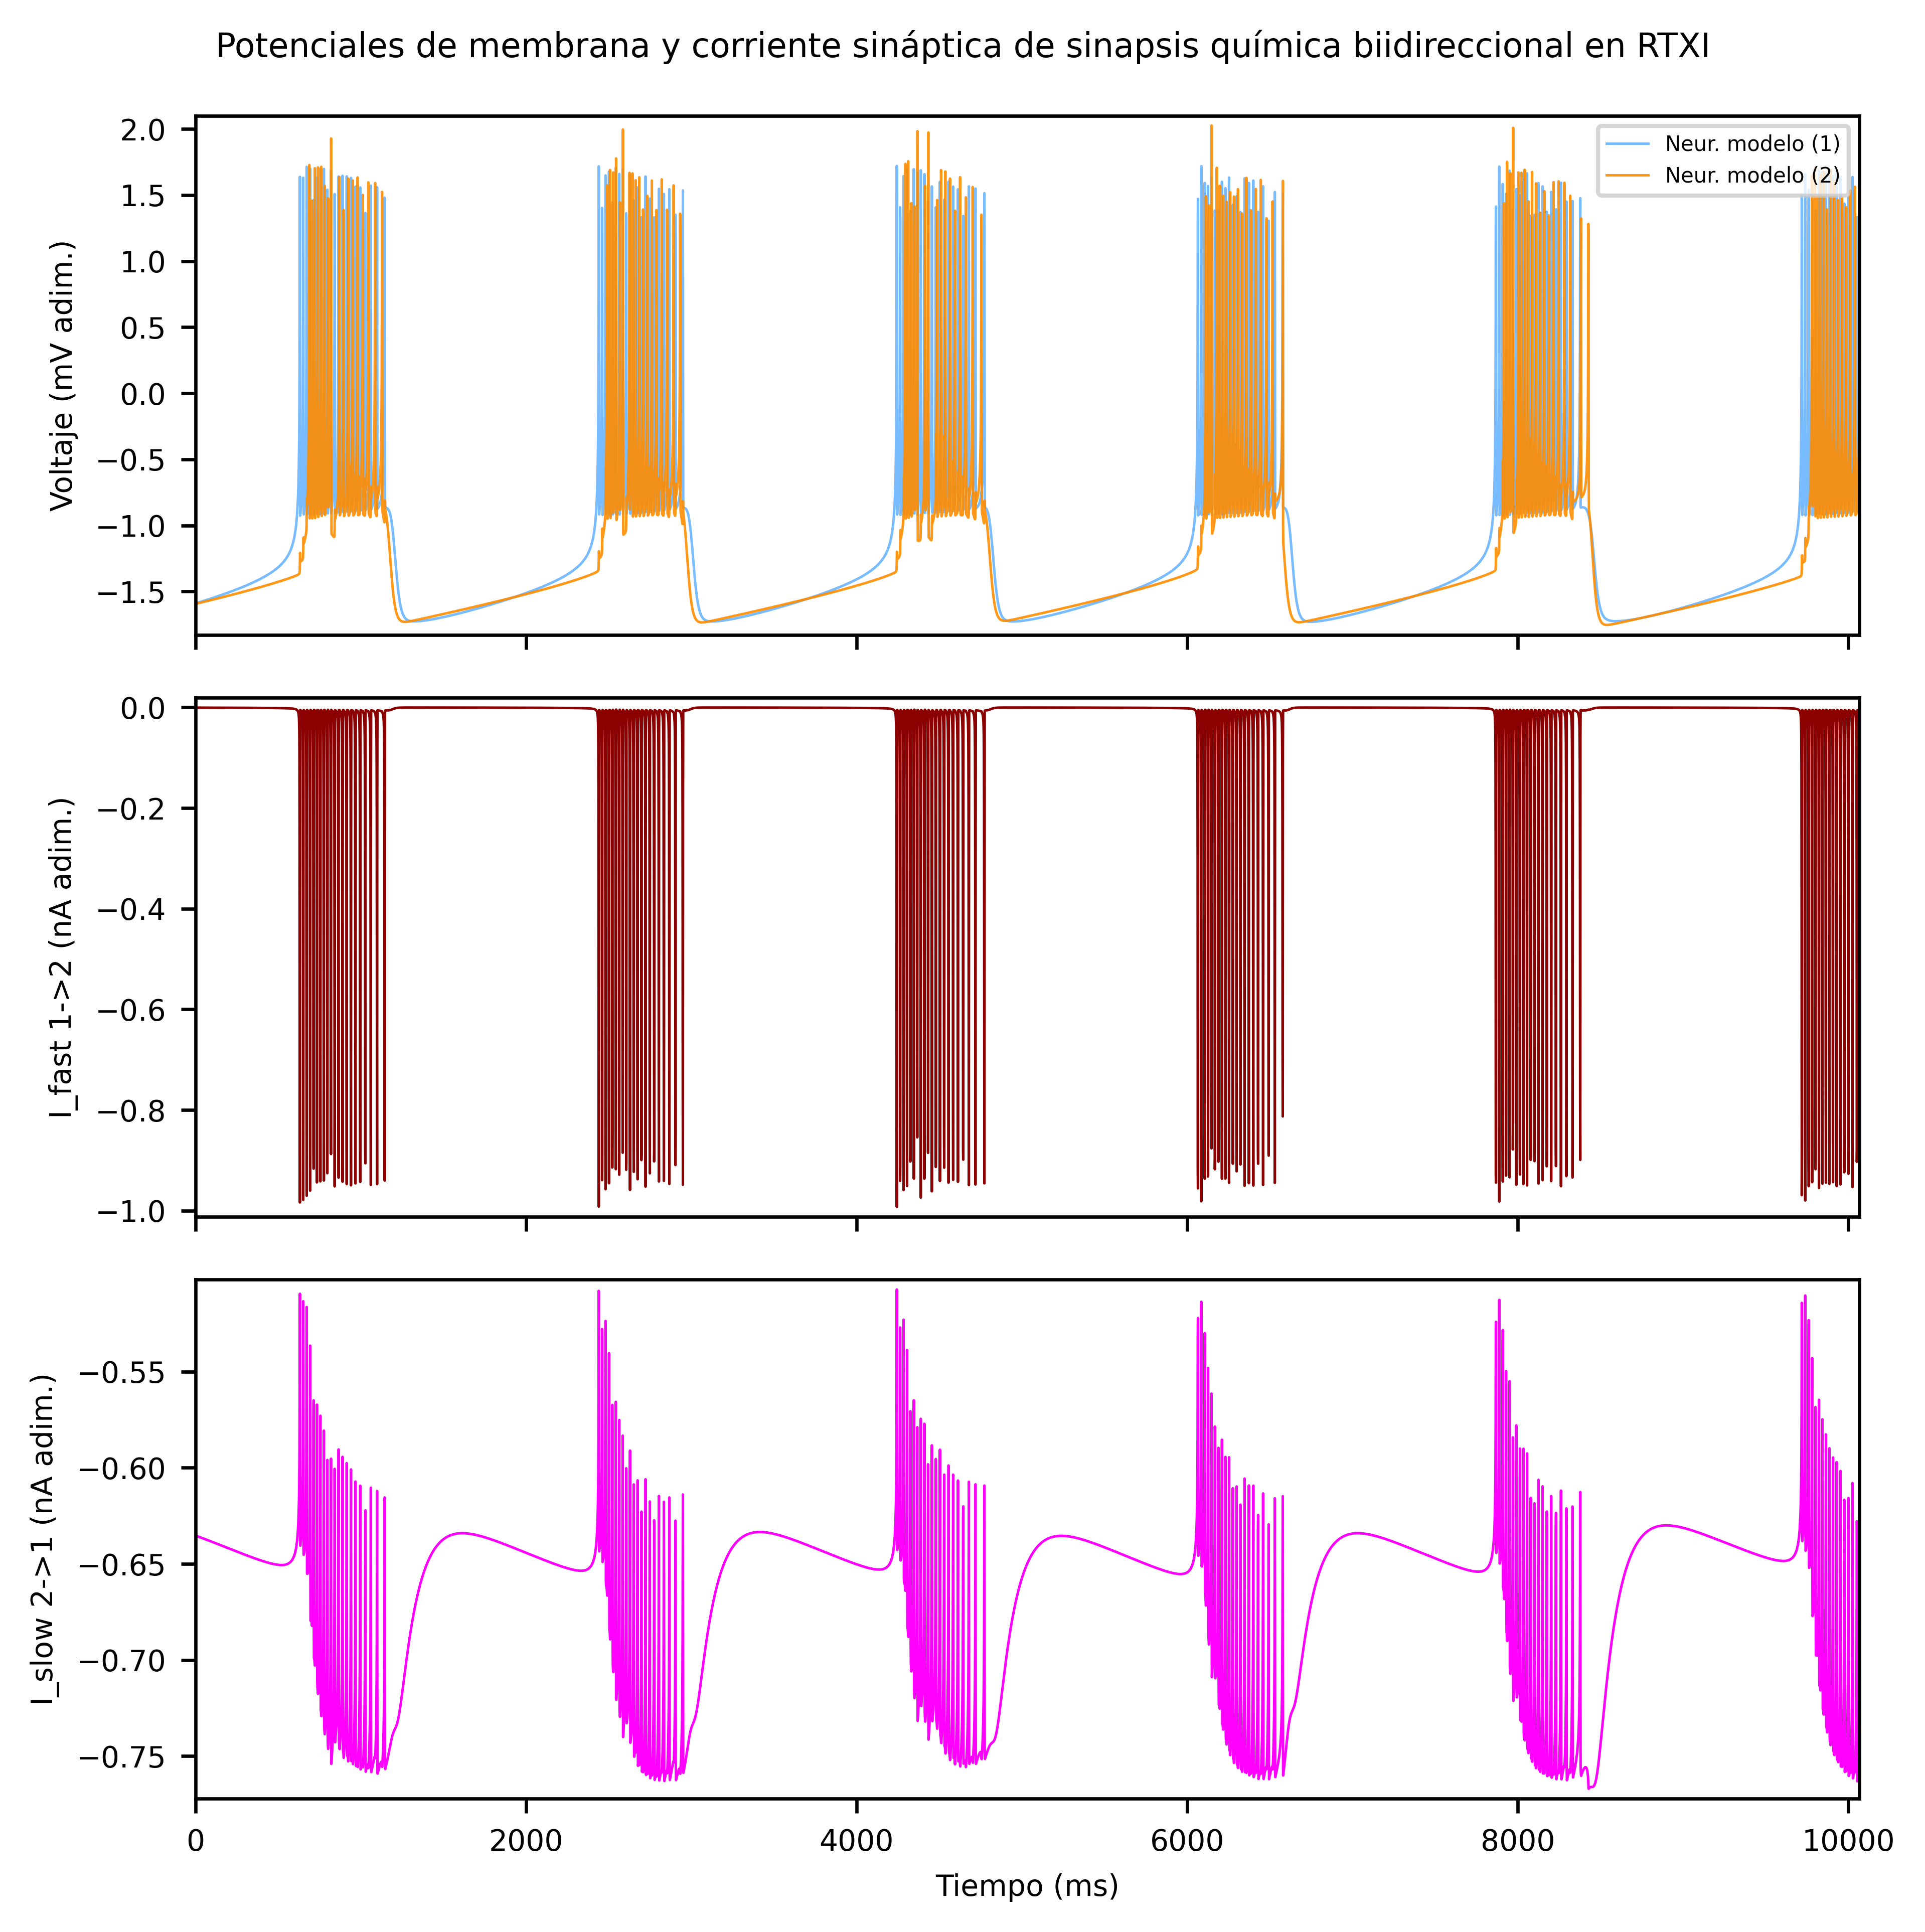
\includegraphics[width=\textwidth, height=0.88\textheight, keepaspectratio]{rtxi_syn_model_ifast_islow_phase}
    \vfill
\end{frame}


\section{Conclusiones y trabajo futuro}



\begin{frame}{Conclusiones}
    \small
    \begin{itemize}
        \item \textbf{Parametrización automática} del modelo de sinapsis química gradual de \textbf{Golowasch et al.} mediante \textbf{BO}.
        \item \textbf{Función de evaluación} (forma + rango de corriente) que orienta \textbf{eficazmente} la búsqueda.
        \item Espacio de búsqueda definido \textbf{cuidadosamente}:
              \begin{itemize}
                  \item Rangos paramétricos \textbf{dinámicos}.
                  \item Estrategias \textbf{anti-\textit{parameter sloppiness}} (\textit{kernel} SE-ARD, reparametrización $R$, escalas logarítmicas).
              \end{itemize}
        \item Implementaciones \textbf{\textit{offline} y \textit{online}} que consegían \textbf{corrientes realistas} (reflejan \textbf{\textit{spikes}} y \textbf{onda lenta} de $\boldsymbol{V_{\mathrm{pre}}}$ de forma separada) y \textbf{dinámicas de acoplamiento} (fase y antifase),  \textbf{convergiendo adecuadamente} en \textbf{tiempos viables} ($\boldsymbol{\sim 30}$ \textbf{s \textit{offline}} y $\boldsymbol{< 16}$ \textbf{min. \textit{online}}) con \textbf{400 evaluaiones}.\\[0.5em]
              Implementación \textbf{\textit{online} sin bloqueos}, necesario para el tiempo real estricto.
        \item Código disponible para el GNB de la UAM.
    \end{itemize}
\end{frame}


\begin{frame}{Limitaciones y trabajo futuro}
    \textbf{Limitaciones:}
    \begin{itemize}
        \item Módulo específico para \textbf{RTXI 2.3}.
        \item \textbf{Imprecisiones menores en extremos} del rango de corriente.
    \end{itemize}
    \vspace{0.8em}
    \textbf{Trabajo futuro:}
    \begin{itemize}
        \item \textbf{Validación con neuronas biológicas} (GNB).
        \item Optimizar \textbf{ambas componentes en ambas direcciones} en la versión \textit{online}.
        \item Funciones de evaluación \textbf{con información temporal más fina}.
        \item Extensión a \textbf{nuevos modelos} neuronales y sinápticos.
    \end{itemize}
\end{frame}


\begin{frame}[plain]
    \vfill
    \centering
    {\LARGE\bfseries\textcolor{azuloscuro}{Muchas gracias por su atención}}\\[2em]
    {\large\textcolor{azuloscuro}{Parametrización del modelo de sinapsis química\\para circuitos neuronales biohíbridos}}\\[2.5em]
    {\normalsize\textcolor{grisoscuro}{Marco Gómez Hernández}}\\[1.0em]
    {\scriptsize\textcolor{grismedio}{Escuela Politécnica Superior — Universidad Autónoma de Madrid}}\\[1.4em]
    {\small\textcolor{grismedio}{Tutor: Pablo Varona Martínez}}
    \vfill
\end{frame}

\end{document}
